% For instructions, 
\documentclass[ reprint, amsmath,amssymb, aps, nofootinbib]{revtex4-2}
\usepackage[T1]{fontenc} %for å bruke æøå
\usepackage[utf8]{inputenc}
\usepackage{graphicx} %for å inkludere grafikk
\usepackage{verbatim} %for å inkludere filer med tegn LaTeX ikke liker
\usepackage{mathpazo}
\usepackage{amsfonts,amsthm}
\usepackage{amsmath}
\usepackage{url}
\usepackage{float}
\usepackage[english]{babel}
\usepackage{listings}
\usepackage[style=numeric]{biblatex}
\usepackage[noend]{algpseudocode}
%\usepackage[style=numeric]{biblatex}
%\usepackage{comment}
\addbibresource{Reference.bib}
\usepackage{subcaption}
\usepackage{listings}
\usepackage{caption}
\usepackage[flushleft]{threeparttable}
\usepackage{array,booktabs,makecell}
\usepackage{multirow}
\usepackage[table,xcdraw]{xcolor}
\usepackage{subcaption}
%\usepackage{algorithm2e}
\usepackage[ruled,vlined,linesnumbered]{algorithm2e}
\usepackage{siunitx}
\usepackage{mathtools}
\usepackage{abstract}
%\usepackage{tocloft}
%\renewcommand{\cftsecleader}{\cftdotfill{\cftdotsep}} 
\usepackage{hyperref}
\usepackage{tikz} 
\usetikzlibrary{shapes,arrows,positioning,automata,backgrounds,calc,er,patterns}
\usepackage{tikz-feynman}
\tikzfeynmanset{compat=1.0.0}
\hypersetup{
    colorlinks=true,
    linkcolor=blue,
    filecolor=magenta,      
    urlcolor=cyan,
}

\usepackage{float}
\newcommand{\subtitle}[1]{%
  \posttitle{%
    \par\end{center}
    \begin{center}\large#1\end{center}
    \vskip0.5em}%
}
\hypersetup{
    colorlinks=true,
    linkcolor=blue,
    filecolor=magenta,      
    urlcolor=cyan,
}

\urlstyle{same}


\renewcommand{\vec}[1]{\mathbf{#1}} % \vec gives bold text instead of arrow
\DeclareMathOperator*{\E}{\mathbb{E}}



\begin{document}
\begin{titlepage}
\centering
\vspace*{2cm}


%{\Large Higgs boson classification using multiple classification methods}
{\Large\bfseries Deployment of unsupervised learning in a search for new physics with ATLAS Open Data}

\vspace{1cm}
{\Large Testing of auto encoder for semi unsupervised learning}

\vspace{1cm}
{\large Sakarias Frette}

\vspace{1cm}
{\bfseries Spring 2022}
\vspace{0.5cm}

\begin{center}
\begin{abstract}

\end{abstract}
\end{center}
\vspace{2.5cm}

{\itshape University of Oslo}
\end{titlepage}
\clearpage
\newpage
\mbox{~}
\clearpage
\newpage

\setcounter{tocdepth}{1}
\tableofcontents




\section{Introduction}
The standard model is arguably the best model ever created by man, showing remarkable accuracy comparing with experiments. Its crown jewel was discovered in 2012 by both ATLAS\footnote{Paper from ATLAS collaboration can be found \href{https://arxiv.org/abs/1207.7214}{here}.} and CMS\footnote{Paper from CMS collaboration can be found \href{https://arxiv.org/abs/1207.7235}{here}.} at CERN. There has however not been any new particle discoveries since the early 70's, and this is somewhat alarming. The standard model has several issues, some of them includes explanation of dark energy, cosmic inflation, the hierarchy problem and no including of gravity. \par 
This leads scientists to look beyond the standard model, and there are several models proposed, such as dark matter candidates, extra vector bosons and super symmetry. Attempts are made by multiple collaborations to discover evidence for these models, and there are several obstacles to overcome, such as method of analysis and sufficient amount of data. With the impressive progress of machine learning software such as Tensorflow\cite{tensorflow2015-whitepaper}, machine learning methods have become more and more popular as possible methods  to use for new physics. \par 
In the last decade machine learning has excelled from being tedious and hard to program to become available to almost everyone. It's scale-ability and ability to discover hidden structure in large datasets makes it an intriguing candidate to use on data from the Large Hadron Collider. One possible candidate is semi unsupervised learning, which is done by an auto encoder. The idea is to train a model-independent algorithm on only background, with the hope that what ever new physics that is in the data is detected, without knowing what it is.  This machine learning model is the method of choice for this report. \par
\\
This report is structured in a theory, implementation, results and discussion, and conclusion section. In the theory section the necessary theory is introduced, with respect to both data, method of analysis and choice of evaluation. In the implementation section I discuss data handling , with respect to cuts, event selection, scaling and feature choices, choice of hyper parameters for grid search and the software and api's used for training and tuning. In the results and discussion section I display the results and discuss them as as well as distinct observations. In the conclusion I summarize my findings. 


\section{Theory}
Some of theory sections about anomaly detection and machine learning algorithms are based on previous work done in other courses, such as \cite{FYSSTK} and \cite{ML_PROJ}.

\subsection{Anomaly detection}

Anomaly detection is a tool with a wide range of uses, from time series data, fraud detection or anomalous sensor data. Its main purpose is to detect data which does not conform to some predetermined standard for normal behavior. The predetermined standard varies from situation to situation, and can be set by the context it self, and what is expected as an anomaly. Anomalies are typically classified in three categories\cite{anom_detec}:
\begin{enumerate}
    \item Point anomalies
    \item Contextual anomalies
    \item Collective anomalies
\end{enumerate}

For the purpose of this report we will mostly consider collective anomalies, as anomalies in the standard model has to be collective to claim anything due to noise etc. \par 

In high energy physics we can, using machine learning, separate anomaly detection into two categories, supervised and unsupervised searches. 

\begin{figure}[H]
    \centering
    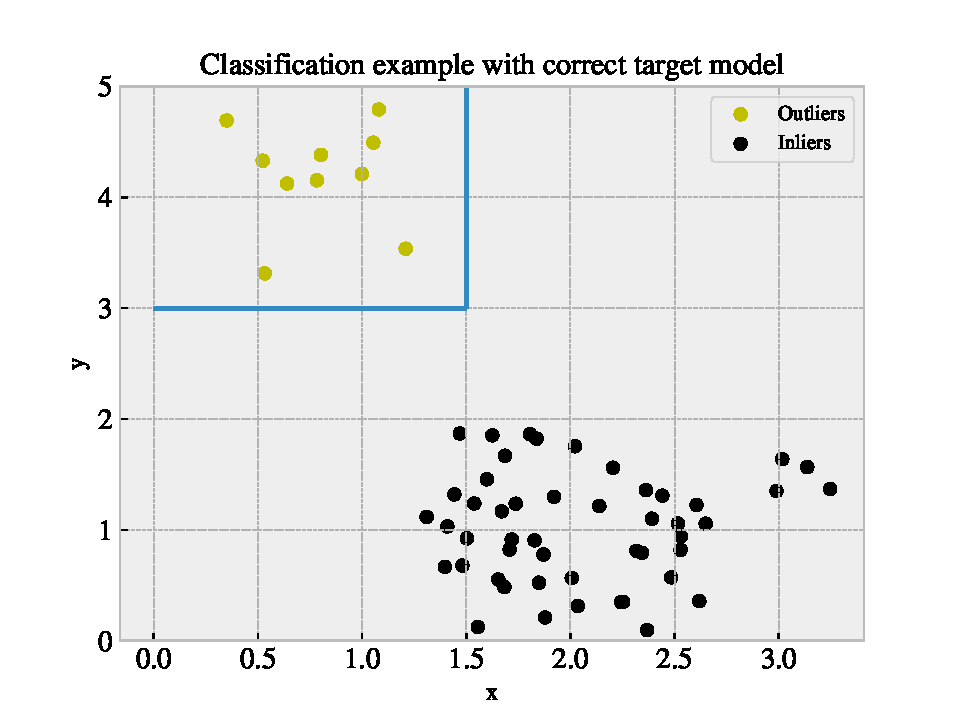
\includegraphics[width=0.49\textwidth]{figures/theory/correct_class.pdf}
    \caption{Example of supervised classification of anomaly where the target model is correct. Here the machine learning model manages to correctly identify the anomalies. }
    \label{fig:corr_class}
\end{figure}

\begin{figure}[H]
    \centering
    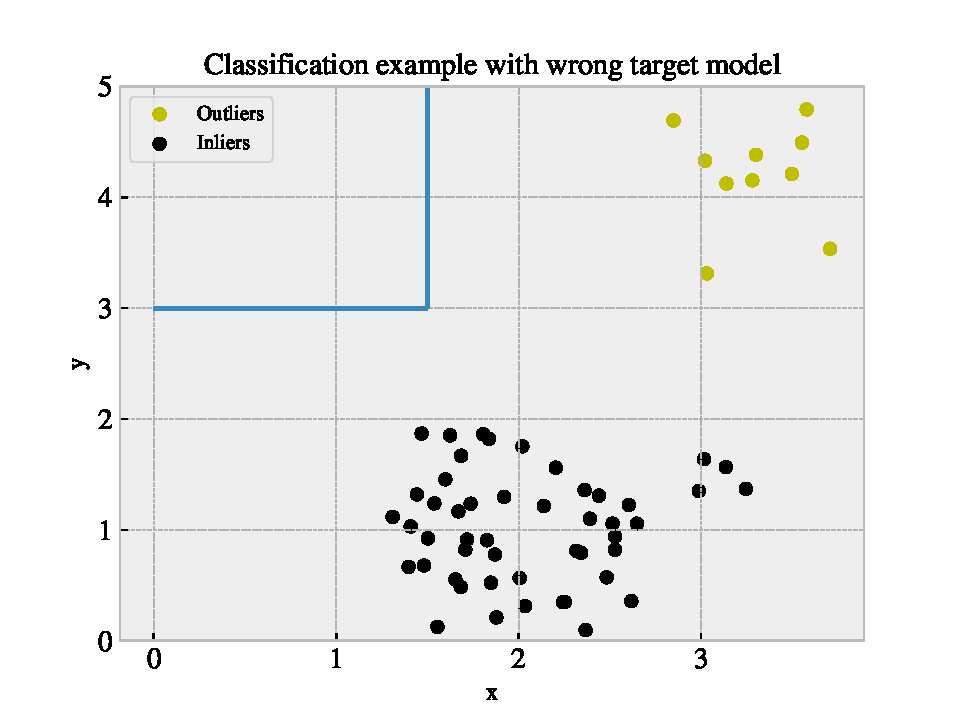
\includegraphics[width=0.49\textwidth]{figures/theory/wrong_class.pdf}
    \caption{Example of supervised classification of anomaly where the target model is wrong. Here the machine learning model manages to wrongly identify the anomalies. }
    \label{fig:wrong_class}
\end{figure}

In figure \ref{fig:corr_class} we see an example of supervised classification. Because the model trained to recognize certain anomalies that are in the data set in manages very well to classify them. In figure \ref{fig:wrong_class} we do however see that the same model does not find any anomalies, as they are completely different from the ones it trained on. 

\begin{figure}[H]
    \centering
    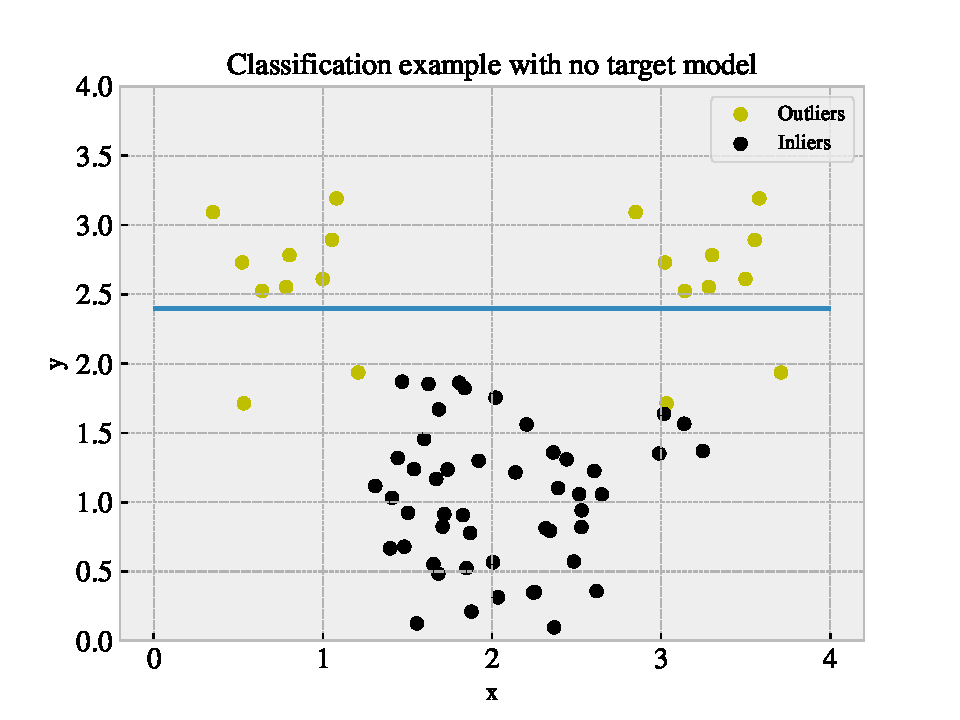
\includegraphics[width=0.49\textwidth]{figures/theory/unsuper.pdf}
    \caption{Example of unsupervised classification of anomaly with no target model. Here the machine learning model manages to with good precision identify the anomalies. }
    \label{fig:unsup_class}
\end{figure}

In figure \ref{fig:unsup_class} we have an example of unsupervised learning. Here we do not tell what is anomalies and what is background. Note that the unsupervised classifier does not classify correctly every anomaly, and the grade of which it does vary from model to model, and from dataset to dataset. 

\subsection{Beyond standard model physics}

In the context of high energy physics, collective anomalies would be new physics with both do and do not have a model for. Such anomalies could be super symmetric particles\cite{JMLR:v18:16-558}, new vector bosons or dark matter particles, as well as many other candidates. These types of searches require enormous amounts of data, and both supervised and unsupervised methods are tried continuously to see if there are "hidden" relations in the data that can separate the known standard model from the unknown new physics.\par 
The methods have their strengths and weaknesses, and should be deployed with this in mind. A supervised model will always be better to classify and separate distribution of background and signal events, and if the signal actually exists in the data from the detector, it will give better accuracy than any (semi-) unsupervised methods. \par 
In the event that some signal actually exist in the data from the detector that we do not have a model for, a supervised model will not be able to recognize it purely as a signal, whilst the unsupervised might claim that there is something other than SM background. The certainty of the results will vary with different models, but in the case of an auto encoder, this is due to the fact that it will only recognize background events that is has trained on, and not any new physics. The drawback with using unsupervised methods in high energy physics, or other fields with multiple anomaly candidates, is that you cannot know what the signal is, only that is it not background. \par 



\subsection{Stacked auto encoder}
One method to attack the anomaly detection problem is the so called (stacked) auto encoder. The idea is based on reconstruction, and has been implemented for denoising of images, image compression, and anomaly detection. An auto encoder is a subgroup of feed forward neural networks, and the goal is to compress the information into fewer variables, called the latent space, which then can explain much of the data through decoding that information. This allows the algorithm to learn the most important components of the data. An illustrative image of an auto encoder is shown below. 

\begin{figure}[H]
    \centering
    \includegraphics[width=0.49\textwidth]{figures/theory/autoencoder-architecture.png}
    \caption{The architecture of an autoencoder with image reconstruction as the example use. \href{https://lilianweng.github.io/posts/2018-08-12-vae/}{Source}, accessed 28.04.22}
    \label{fig:auto_en_archi}
\end{figure}

We see here in figure \ref{fig:auto_en_archi} that the input data is deconstructed through an encoder to a lower dimensional space called the latent space, depicted here as \textbf{z}, and then reconstructs the data with the decoder. It is important to note that the number of layers, nodes per layer and activation function per layer for the encoder does not need to match the structure of the decoder. The only requirement is that the input and output layer has the same shape. The end result is the reconstructed data \textbf{x'}. The training of the model is parameterized in the following way. We define the decoder as 

\begin{equation*}
    \textbf{z} = g_{\xi}(\bf{x}),
\end{equation*}
and the reconstructed information as 
\begin{equation*}
    \textbf{x'} = f_{\theta}(g_{\xi}(\bf{x})),
\end{equation*}

where the parameters $(\xi, \theta)$ are tuned to reconstruct the data as close to the original data as possible. The model then adjusts following the simple mean squared error of the reconstruction and the actual data, given below

\begin{equation*}
    L_{AE}(\xi, \phi)= \frac{1}{N} \sum_{i=0}^{N-1}\bigg( \textbf{x}^i - f_{\theta}(g_{\xi}(\textbf{x}^i))\bigg)^2
\end{equation*}



\section{Implementation}

\subsection{Handling of data}

In appendix \ref{appendix:features} the features used in the data set are listed, with their respective type and description. The data can be separated into two categories, Monte Carlo simulated (MC) data and actual data from a detector. The MC data contain background samples which are standard model processes, and signal samples which are proposed new physics. The actual data is data from the ATLAS detector. The totality of the data used in this report is given as ATLAS Open Data\footnote{Link to ATLAS Open Data \href{https://atlas.cern/resources/opendata}{here}.}. This is a dataset that has been analyzed for new physics, and can thus be released to the public. 

\subsubsection{Cuts, pre-selection and scaling}
To preserve as much information and add as little bias as possible I did very few cuts. The entire data gathering process is biased from the moment the data is collected at the collider, but even then it is good to try to minimize the bias. \par
The first cut I impose is to require "good leptons". This is done by requiring lep\_etcone$20/$lep\_pt $< 0.15$ and lep\_ptcone$30/$lep\_pt $< 0.15$. We then require only two leptons per event. The event selection was done using RDataframe, to speed up the selection\footnote{This code was written by Eirik Gramstad, and can be found \href{https://github.uio.no/zpath/software/blob/eirik-dev/Notebooks/ATLASOpenData/13TeV/RDataFrameToDF.ipynb}{here}.}\par 
I tested two methods of scaling in this report, Min Max Scaling\footnote{More on Min max scaling \href{https://scikit-learn.org/stable/modules/generated/sklearn.preprocessing.MinMaxScaler.html}{here}.} and Standard scaling\footnote{More on Standard scaling \href{https://scikit-learn.org/stable/modules/generated/sklearn.preprocessing.StandardScaler.html}{here}.}\cite{scikit-learn}.

\subsubsection{Choice of features}
The choice of features is a mixture of specification and broadness. In this context specification is defined as information that specify for a given part of the physical system, in this case the leptons. Thus, most of the features are directly related to the leptons. Broadness is in this context defined as information about the rest part of the final state, such as jets, photons or tau leptons. Ideally one would pick as much information as possible for each event, but there is a trade-off between amount of information and size of data, and as consequence, execution time. \par 
The features were picked such that there are no missing values, only 0 or larger than 0. For regular machine learning problems, missing values usually gets replaced by the mean value of the feature. This is however a problem when analysing physics, as such a choice could violate the laws of physics. To avoid this, all features are designed to either have 0 if missing, or sum up the contributions of both missing and present values, given that they represent the same type of information. \par 
An example of this is if we have two jets in one event and three in another, using the transverse momentum of the jets as features. We cannot in the first event input the mean values of all third jet-transverse momentum in the entire dataset, but we could put 0, or sum all the transverse momentum for the jets in the given event into one feature. Another possibility is to only give the count of jets in the event, and there are even more ways to solve this issue. 



 

\subsection{Tuning and training}
For the auto encoder to accurately reconstruct the standard model, the model needs to train on the background MC. However, neural networks are highly susceptible to hyperparameters, which needs tuning. In this project I used Keras-tuner\cite{omalley2019kerastuner} to tune the hyperparameters. The choice of tuner for this report was Hyperband\cite{JMLR:v18:16-558}. It is not well understood how the hyperparameters interact with each other to affect the result, thus there are really no guidelines for approaching this problem. A result of this might be that the choice of hyperparameters seem completely random or strange. The hyperparameters used in the network are the learning rate, the alpha parameter for the LeakyReLU\footnote{More on the LeakyReLU api can be found \href{https://www.tensorflow.org/api_docs/python/tf/keras/layers/LeakyReLU}{here}.} activation function, the activation function for each layer, the amount of nodes per layer and regularization for layer's kernel and output AND . The activation functions used in the hyperparameter grid search where
\begin{itemize}
    \item ReLU
    \item LeakyReLU
    \item tanh
    \item linear
\end{itemize}
whilst the different learning rates that was tested was $[9\cdot 10^{-2}, 9.5\cdot 10^{-2}, 10^{-3}, 1.5\cdot 10^{-3}]$, and the kernel and output regularization constant values were $[0.5, 0.1, 0.05, 0.01]$. The optimizer used for all the models is the ADAM\footnote{More on ADAM optimizer \href{https://www.tensorflow.org/api_docs/python/tf/keras/optimizers/Adam}{here}.} optimizer. \par 
The auto encoder was written using Tensorflow api\cite{tensorflow2015-whitepaper}\cite{chollet2015keras}, using a functional structure\footnote{More on the functional api can be found \href{https://www.tensorflow.org/guide/keras/functional}{here}.}. In practise, this model could just as well have been written as a Sequential model\footnote{More on sequential models can be found \href{https://www.tensorflow.org/guide/keras/sequential_model}{here}.}, but at a cost of flexibility and lack of potential non-linear structure in the architecture. \par 
Certain features where removed, as they did not have a good enough overlap between MC and ATLAS data. All features where checked to ensure as good correspondence as possible, and the figures for all the features can be found in the \href{https://github.com/Gadangadang/FYS5555/tree/main/Project3}{Github repo} for this project, under the "figures/implementation" folder. The features that were chosen to exclude where lep1\_tracksigd0pvunbiased and lep2\_tracksigd0pvunbiased, which are shown below:

\begin{figure}[H]
    \centering
    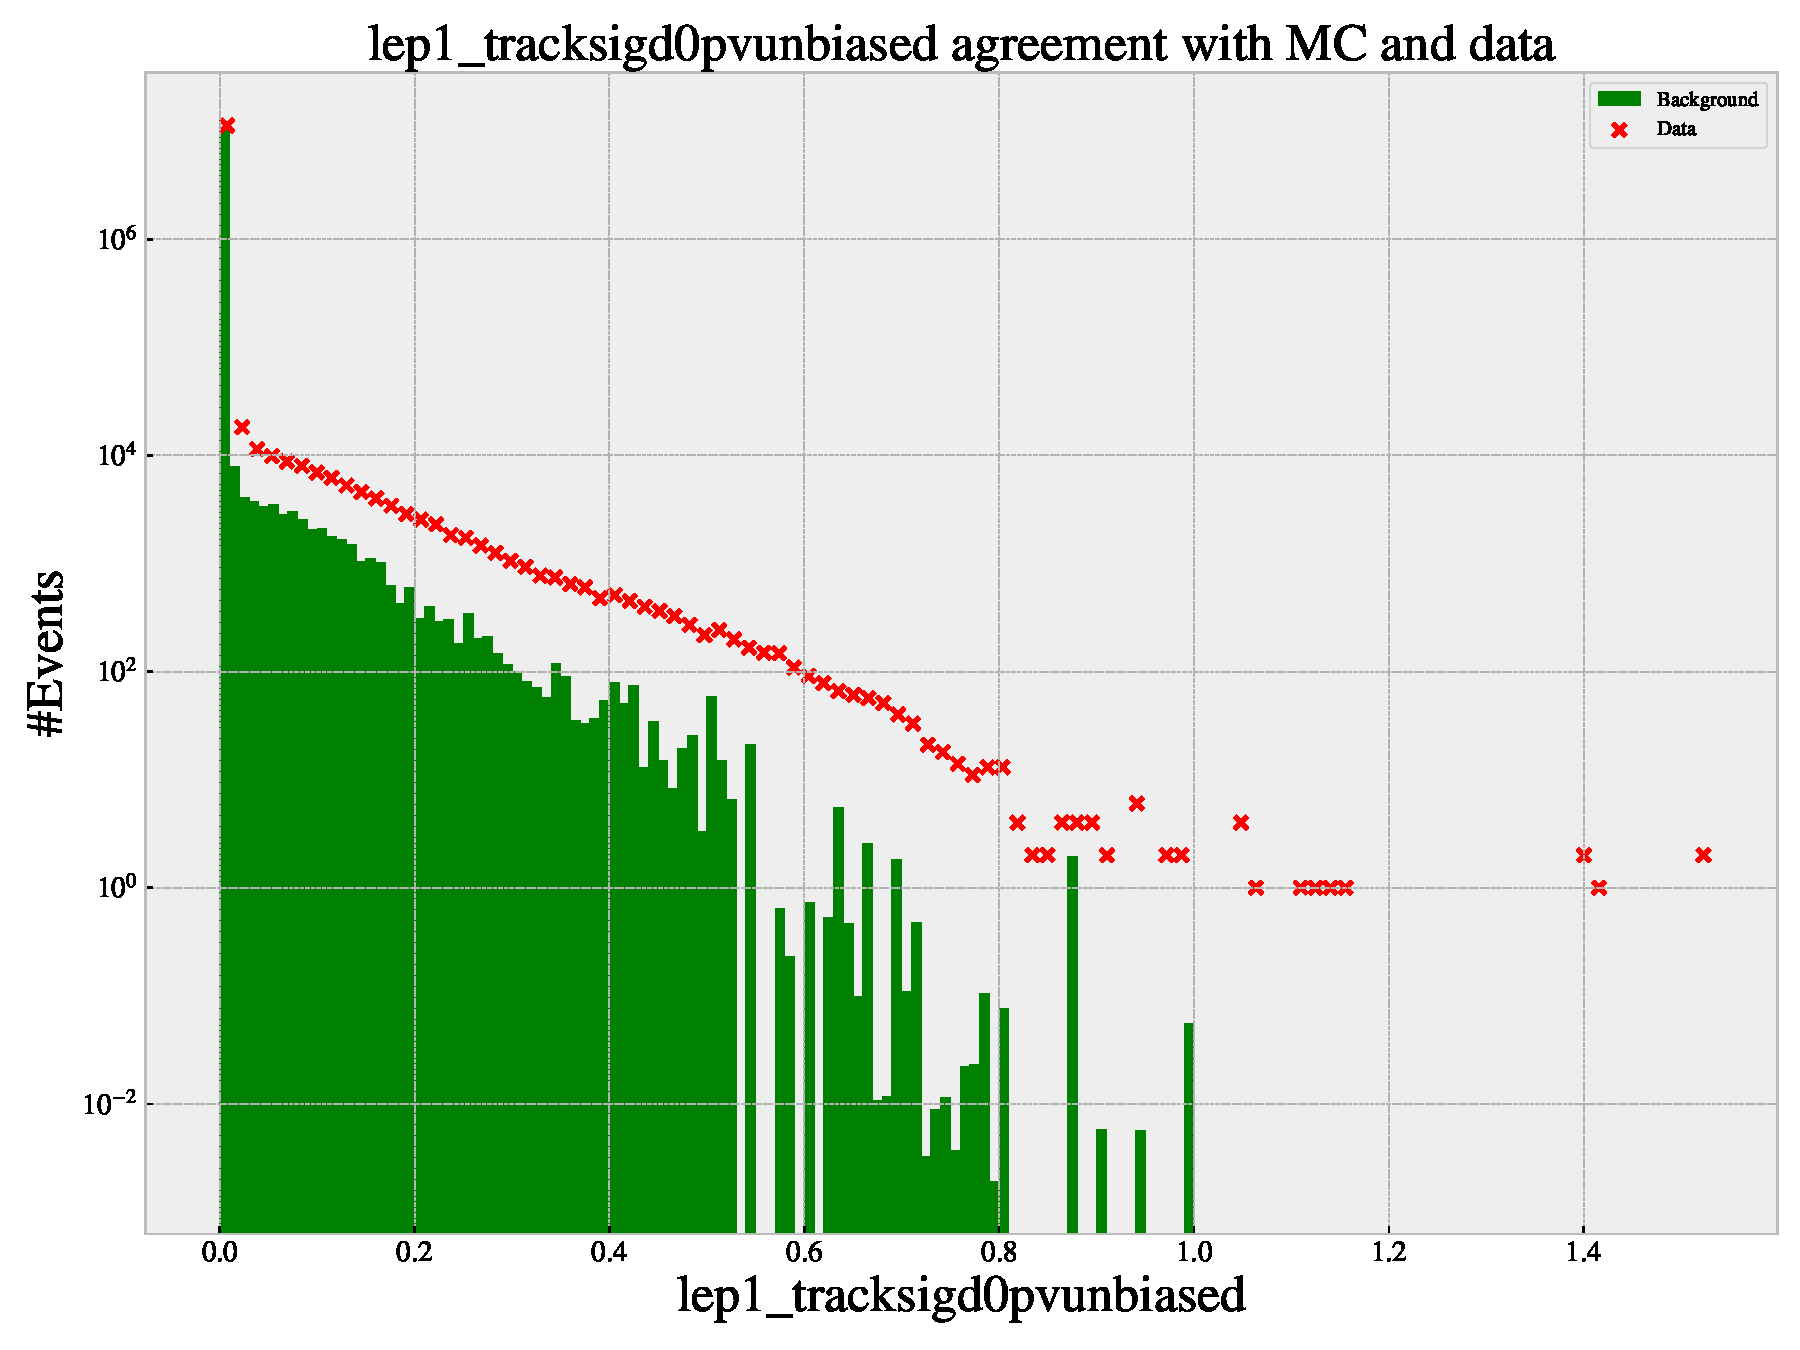
\includegraphics[width=0.46\textwidth]{figures/implementation/lep1_tracksigd0pvunbiased.pdf}
    \caption{Lep1 tracksigd0unbiased histogram for background MC and ATLAS data. }
    \label{fig:lep1sigd0}
\end{figure}

\begin{figure}[H]
    \centering
    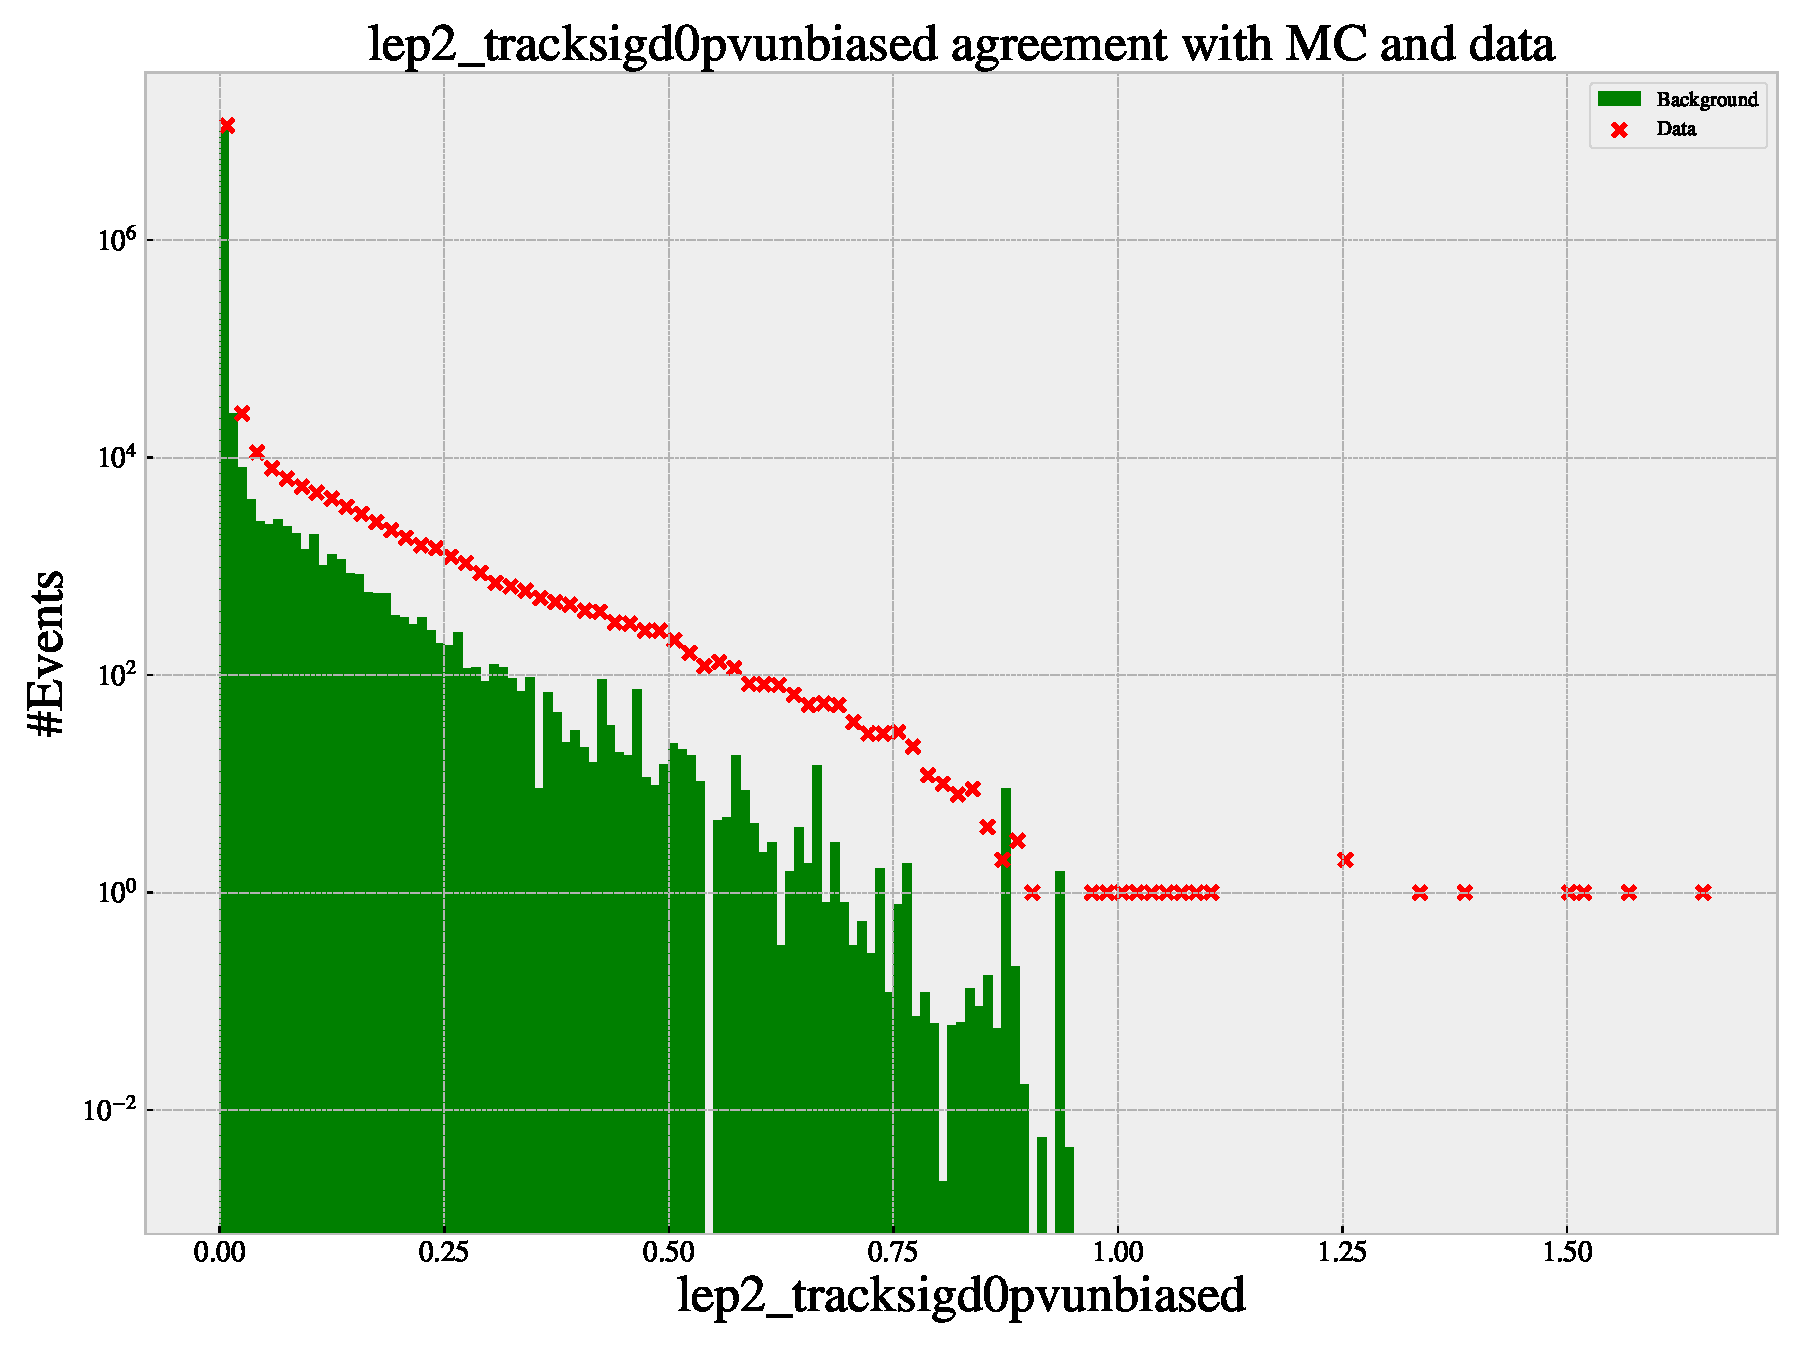
\includegraphics[width=0.46\textwidth]{figures/implementation/lep2_tracksigd0pvunbiased.pdf}
    \caption{Lep2 tracksigd0unbiased histogram for background MC and ATLAS data.}
    \label{fig:lep2sigd0}
\end{figure}


\section{Results and Discussion}

\subsection{The first model}

The first auto encoder model was found with a grid search and is structured as shown in figure \ref{fig:big_ae_plot} below. 

\begin{figure}[H]
    \centering
    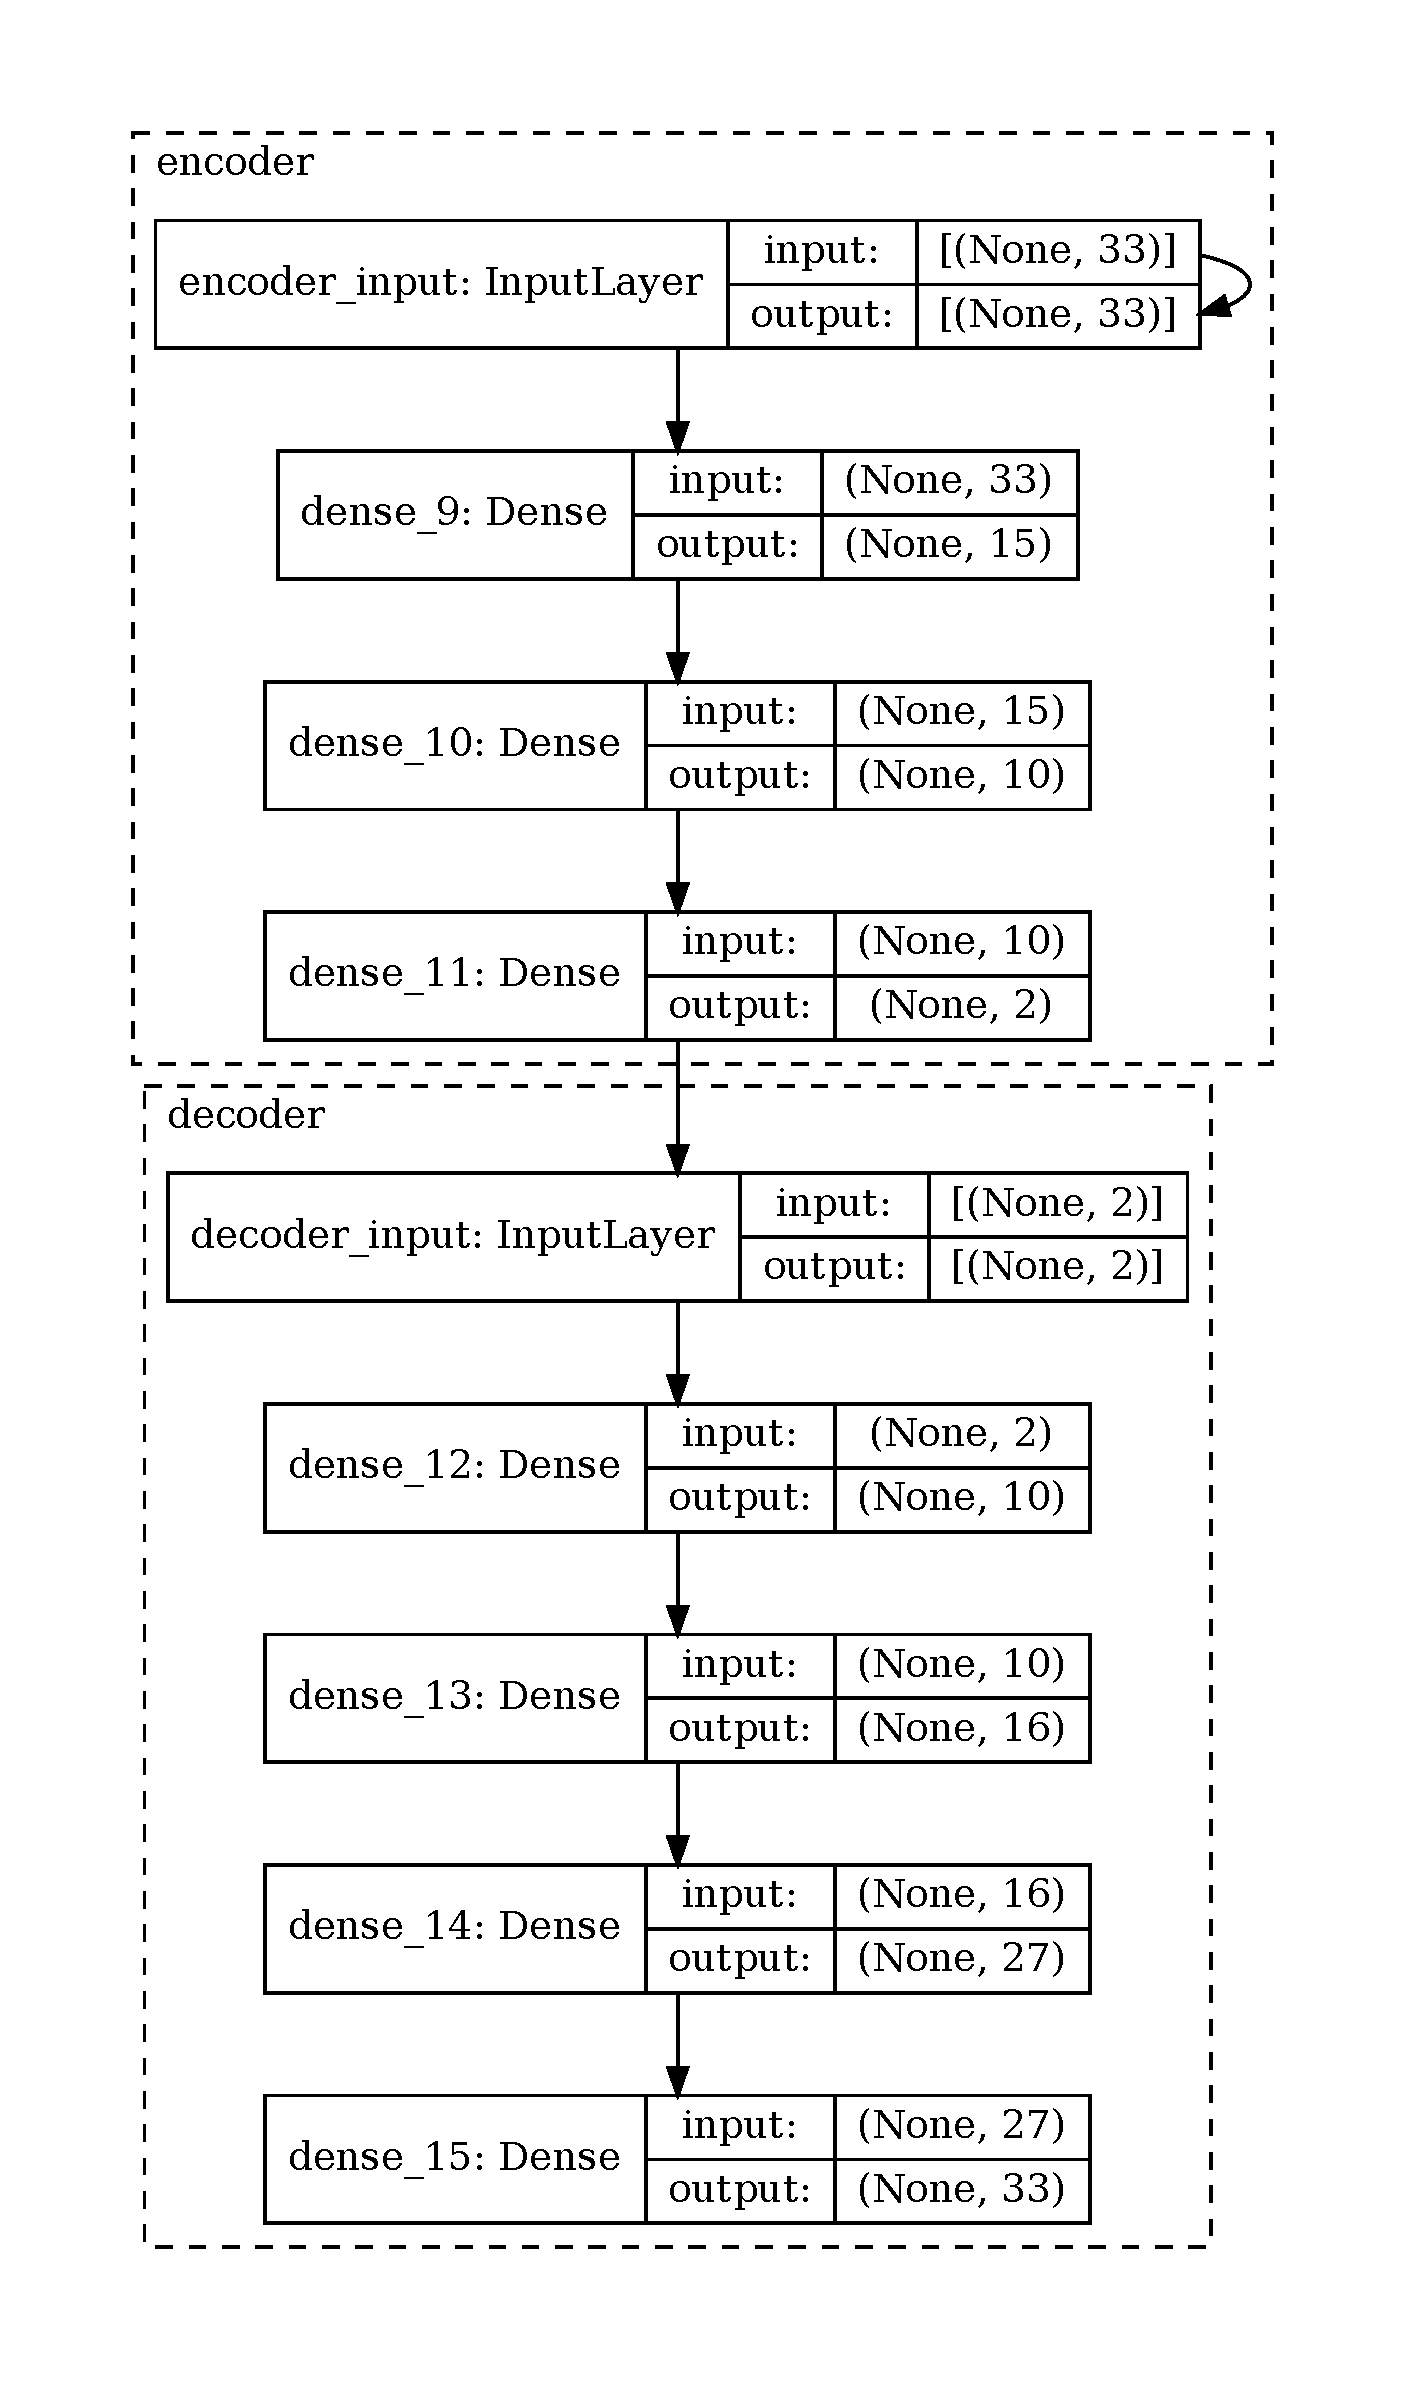
\includegraphics[width=0.46\textwidth]{figures/results/models/ae_model_plot_big_rm3feats.pdf}
    \caption{Auto encoder architecture after grid search. }
    \label{fig:big_ae_plot}
\end{figure}
The grid search gave the optimal hyper parameters as follows: the encoder has the following activation functions: tanh, linear, linear, leakyReLU, and the decoder has the following activation functions: relu, leakyReLU, tanh, and linear. The optimal learning rate was 0.0015, the optimal kernel regularizer was 0.05, the optimal activity regularizer was 0.5 and the optimal alpha for the leakyReLU was 1. These hyper parameters was found after around 30 minutes of searching, and then stopped, as it appeared that the validation MSE did not improve much. Thus, there are most likely a better set of hyper parameters that could get an even lower validation MSE. \par 
The reconstruction error of ATLAS data is shown in figure \ref{fig:data_b_big_pred}.

\begin{figure}[H]
     \centering
         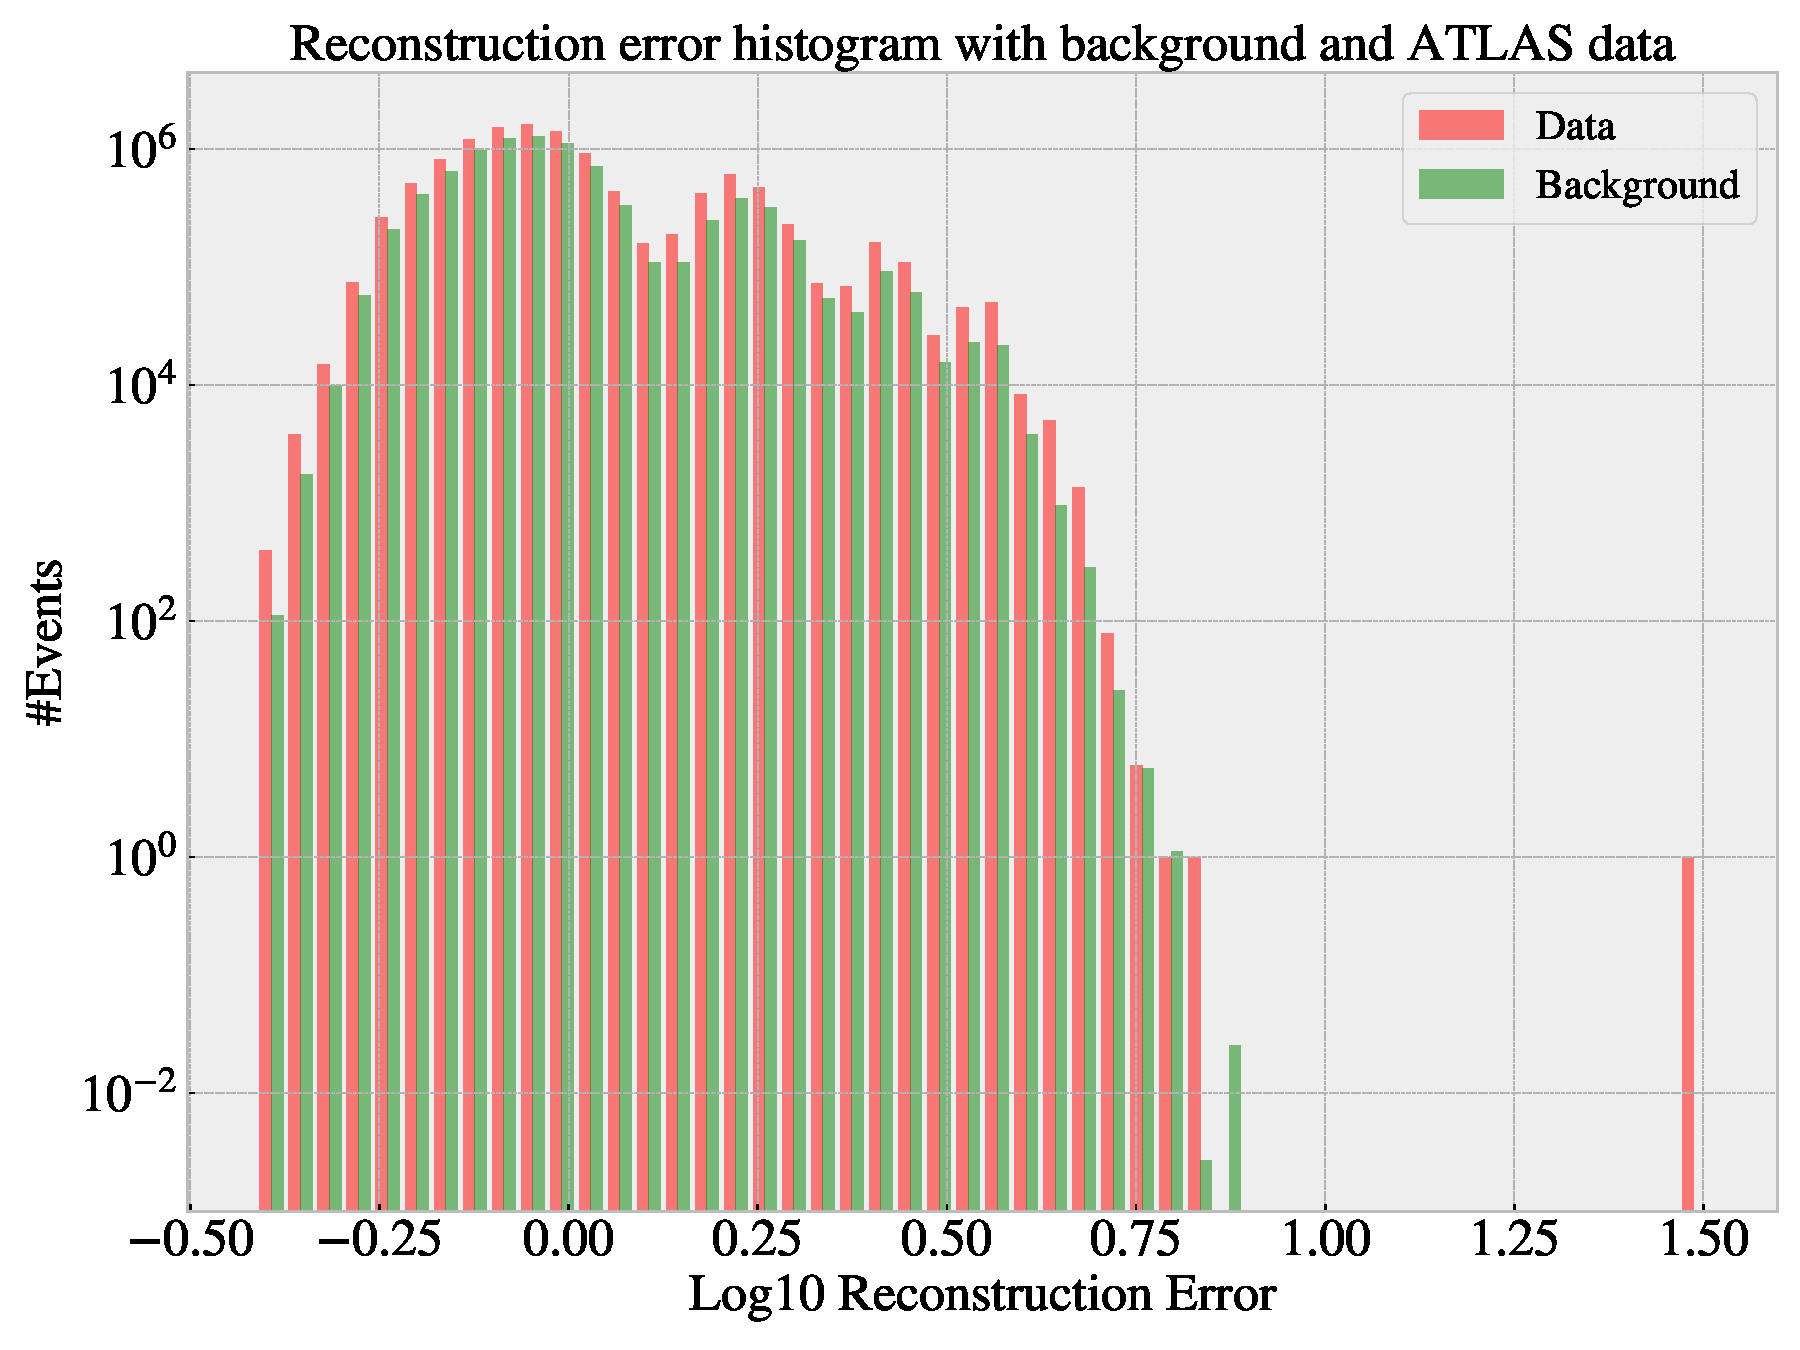
\includegraphics[width=0.46\textwidth]{figures/results/predictions/b_data_recon_big_rm3_feats.pdf}
         \caption{Histogram showing reconstruction error for ATLAS data and background MC for big auto encoder. }
     \label{fig:data_b_big_pred}
\end{figure}

In figure \ref{fig:data_b_big_pred} we see that the auto encoder gets a good overlap of reconstruction error between ATLAS data and background MC. This is in accordance with the fact that the ATLAS collaboration have with very high certainty only found SM data in the ATLAS Open Data. Using all the signal MC samples, I can test if the classifier can distinguish new physics signal MC from SM processes by mere reconstruction. The reconstruction error is shown in figure \ref{fig:s_b_big_pred_allsig}.


\begin{figure}[H]
     \centering
         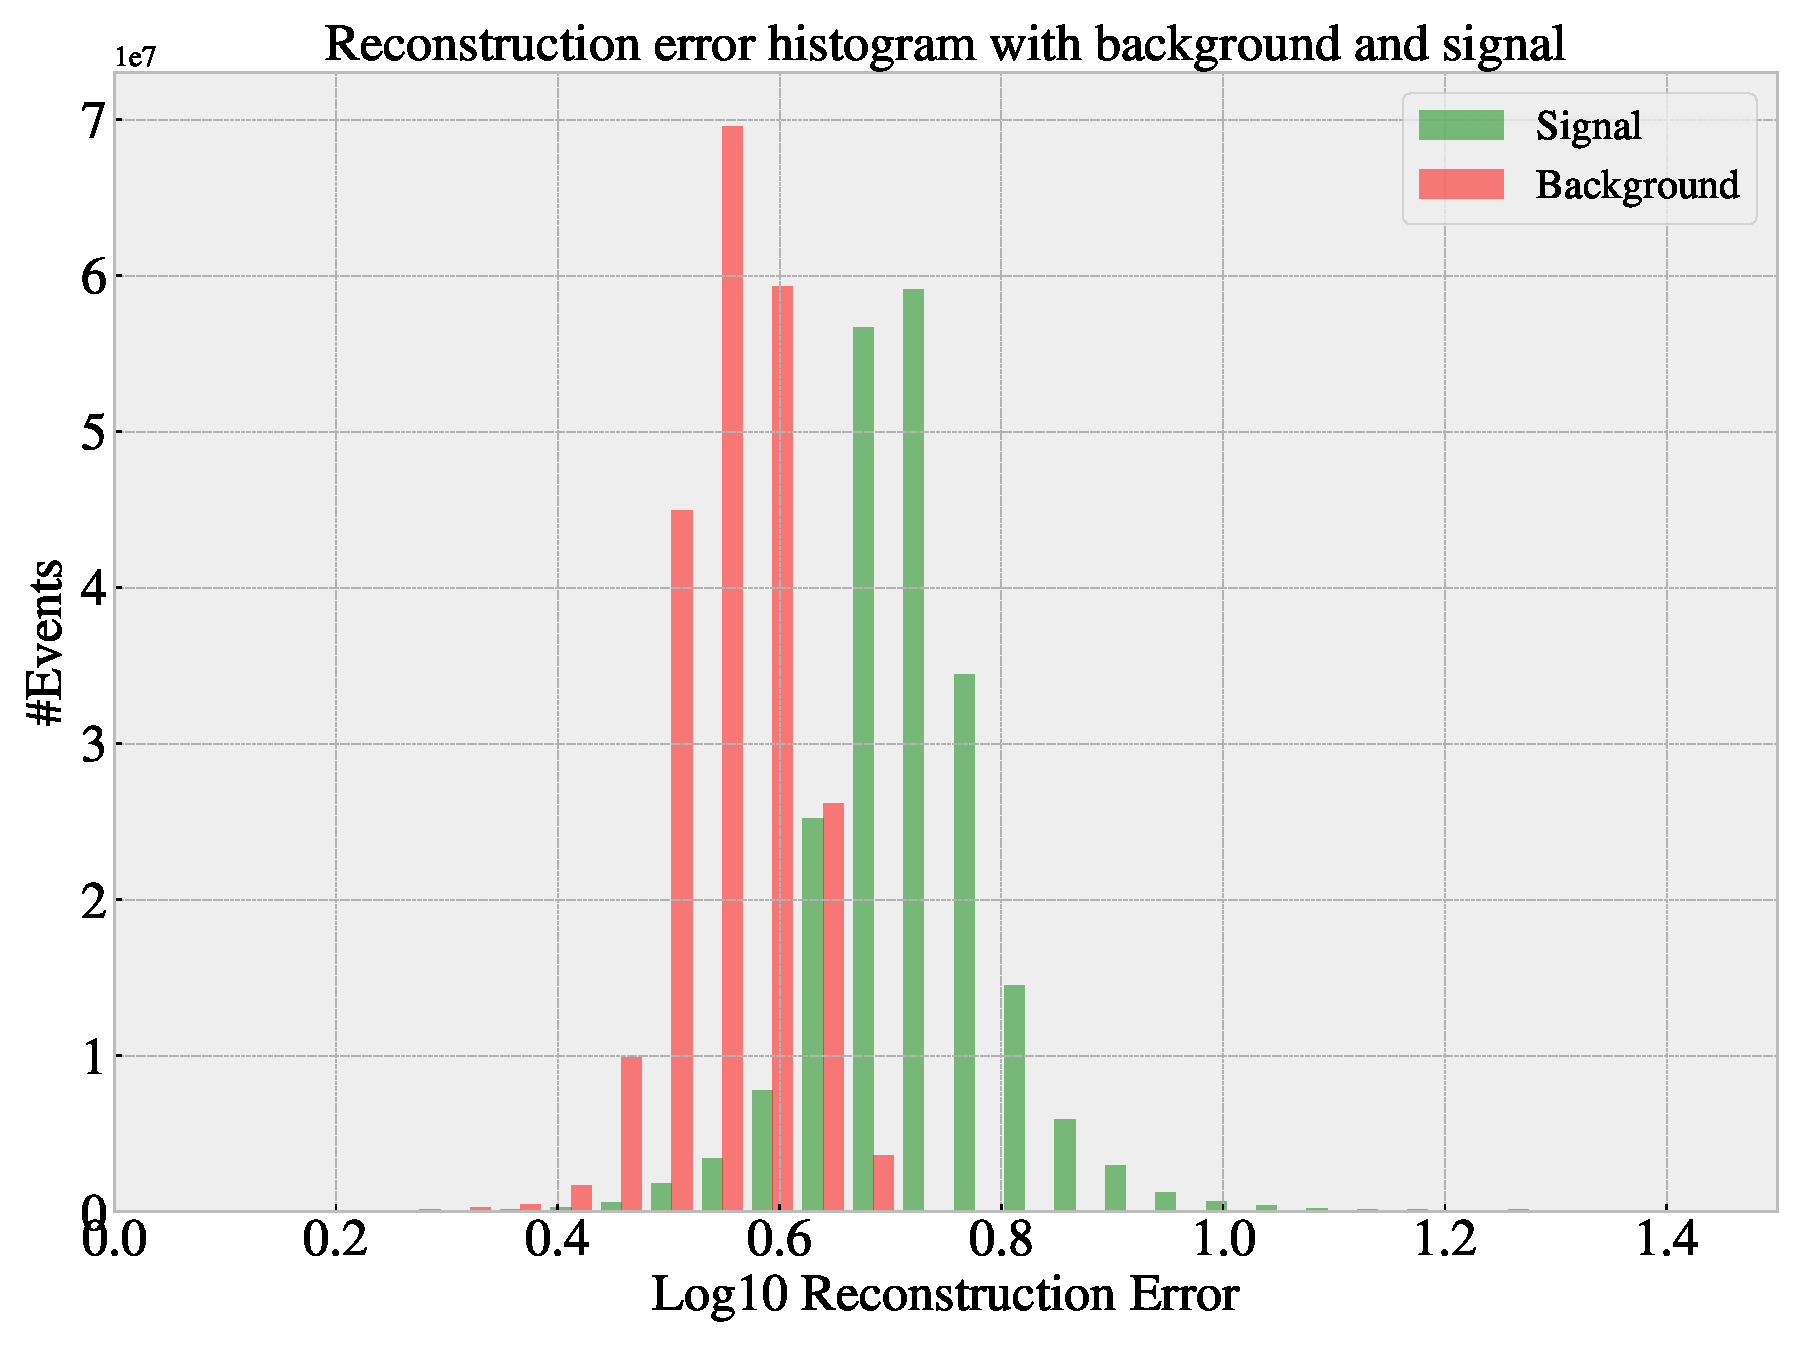
\includegraphics[width=0.46\textwidth]{figures/results/predictions/b_s_recon_big_rm3feats_allsig_nolog.pdf}
    \caption{Reconstruction error of background MC and signal MC for big auto encoder with all signal samples.  }
    \label{fig:s_b_big_pred_allsig}
\end{figure}


\begin{figure}[H]    
    
    \centering
         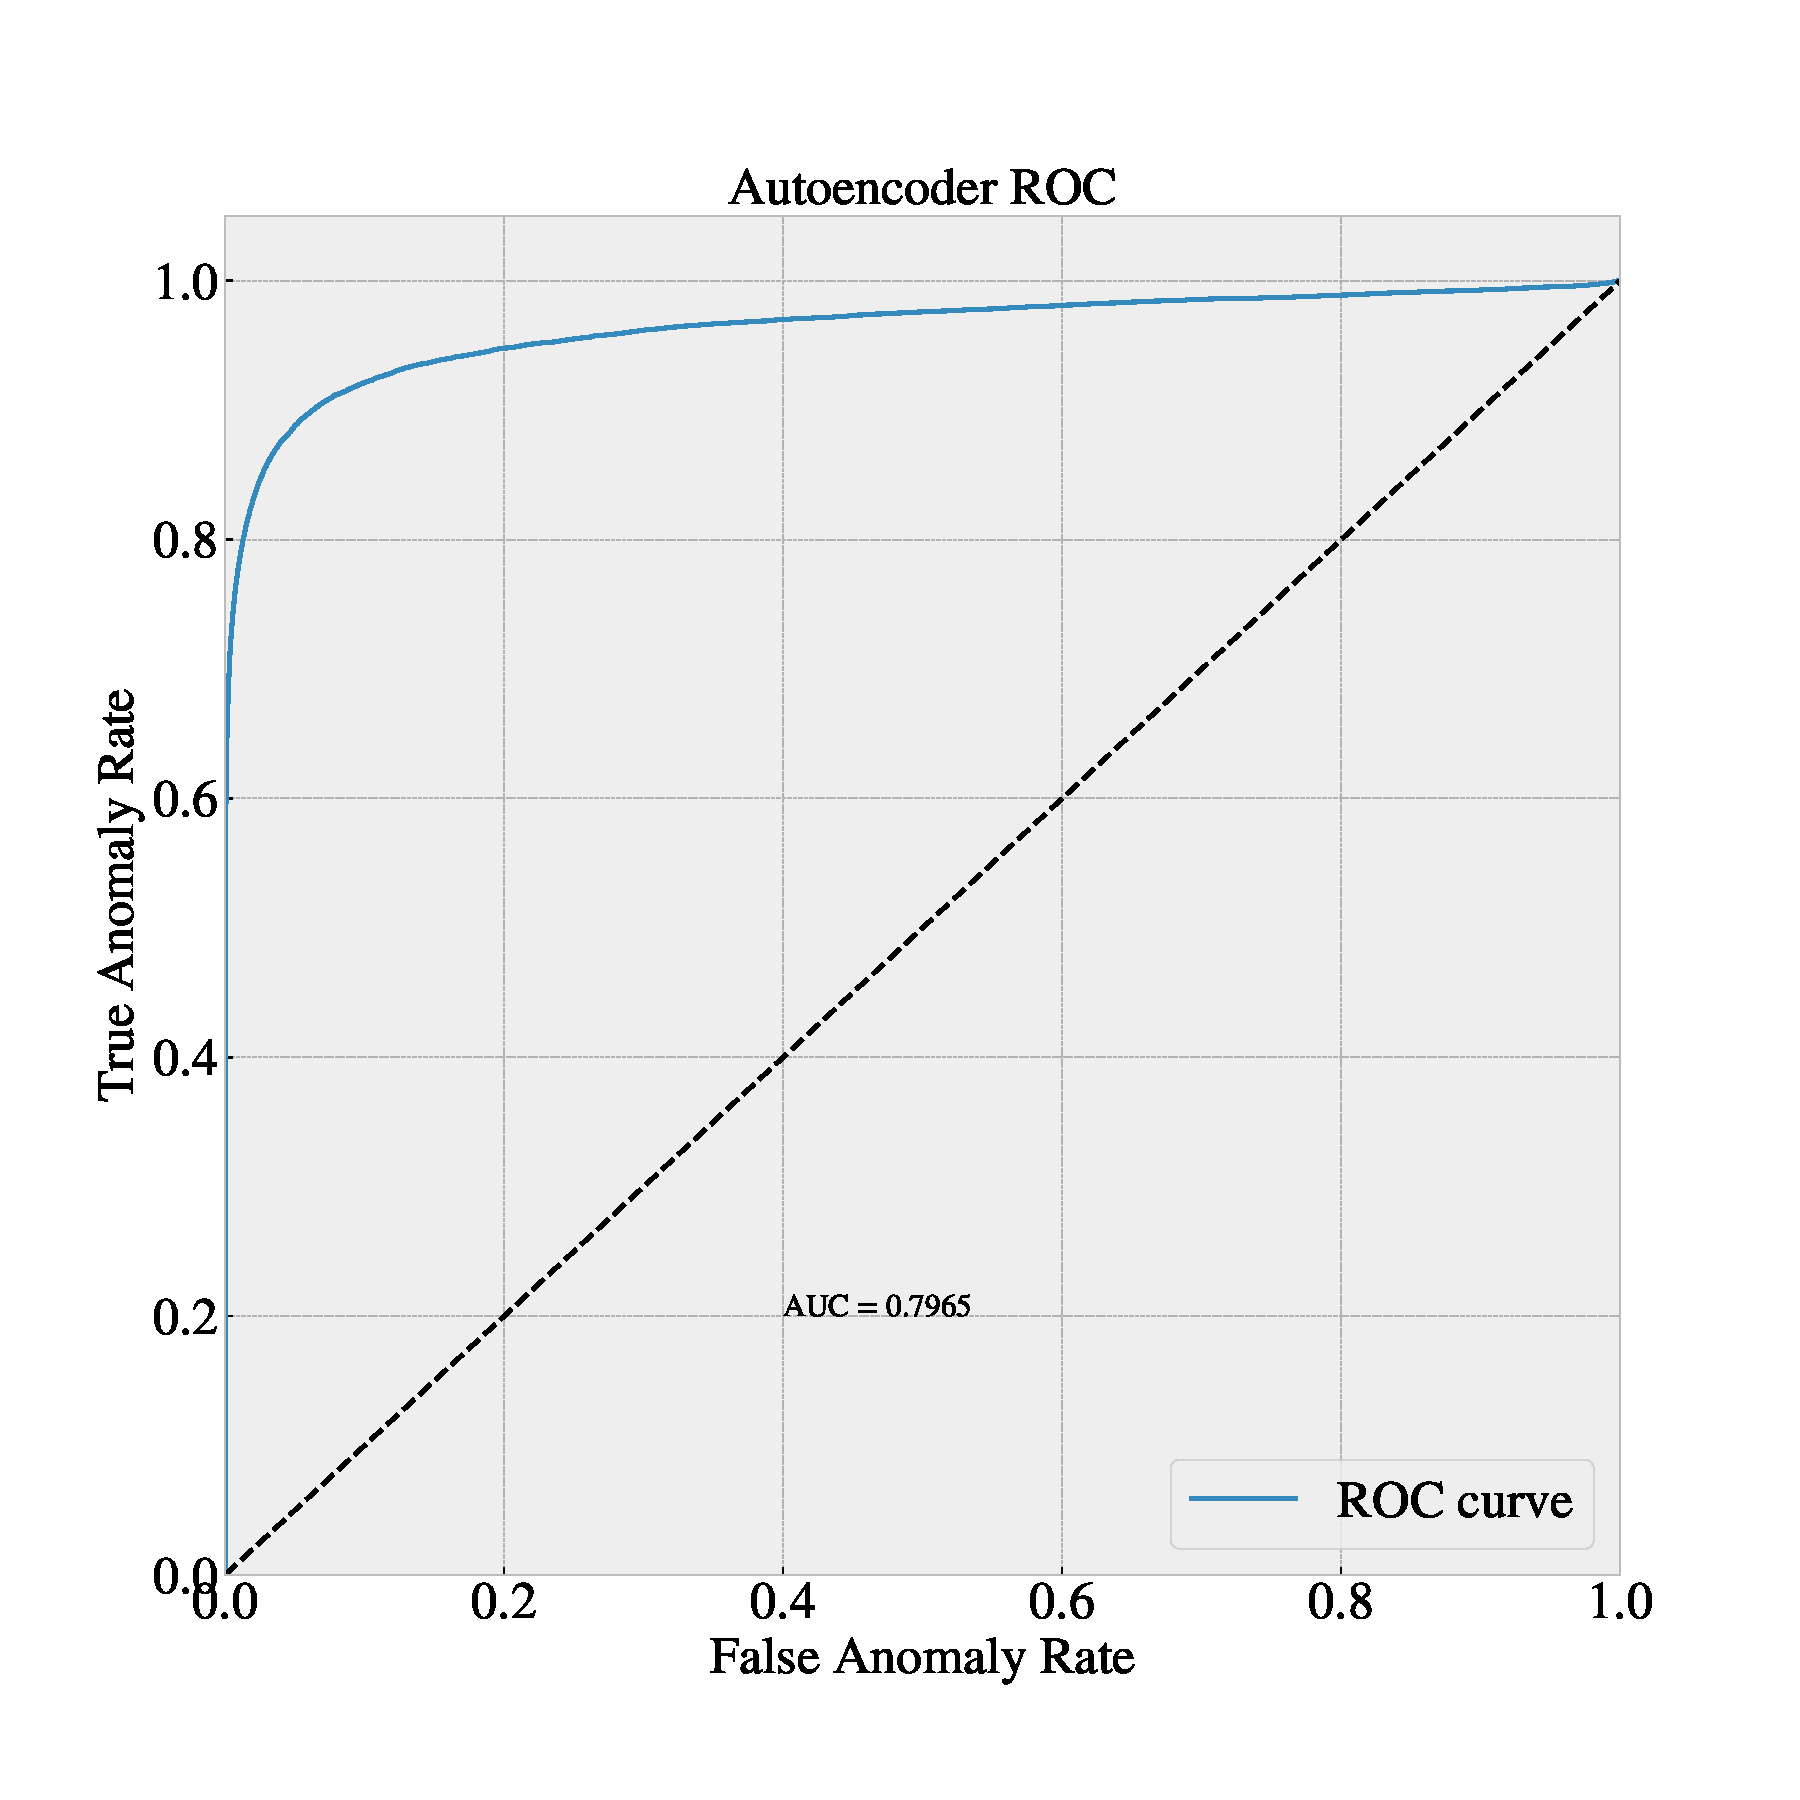
\includegraphics[width=0.46\textwidth]{figures/results/rocs/b_s_roc_curve_big_rm3feats_allsig.pdf}
         \caption{ROC curve signal MC and background MC for big auto encoder with all signal samples.}
         \label{fig:s_b_big_roc_allsig}
\end{figure}


From these results in figure \ref{fig:s_b_big_pred_allsig} and \ref{fig:s_b_big_roc_allsig} it appears that the auto encoder very well manages to separate signal from background, having only been shown background MC. However, there is some problems with these results. The Randall-Sundrum Graviton to dimuons samples in the signal MC were given with very high weights compared to the Graviton to dielectrons samples, which highly indicates that the data samples are corrupt somehow. Thus we have to check the reconstruction error on signal MC without the Randall-Sundrum Graviton samples. This is shown in figure \ref{fig:roc_sig_big_allsig_nogmumu}.


\begin{figure}[H]    
     \centering
    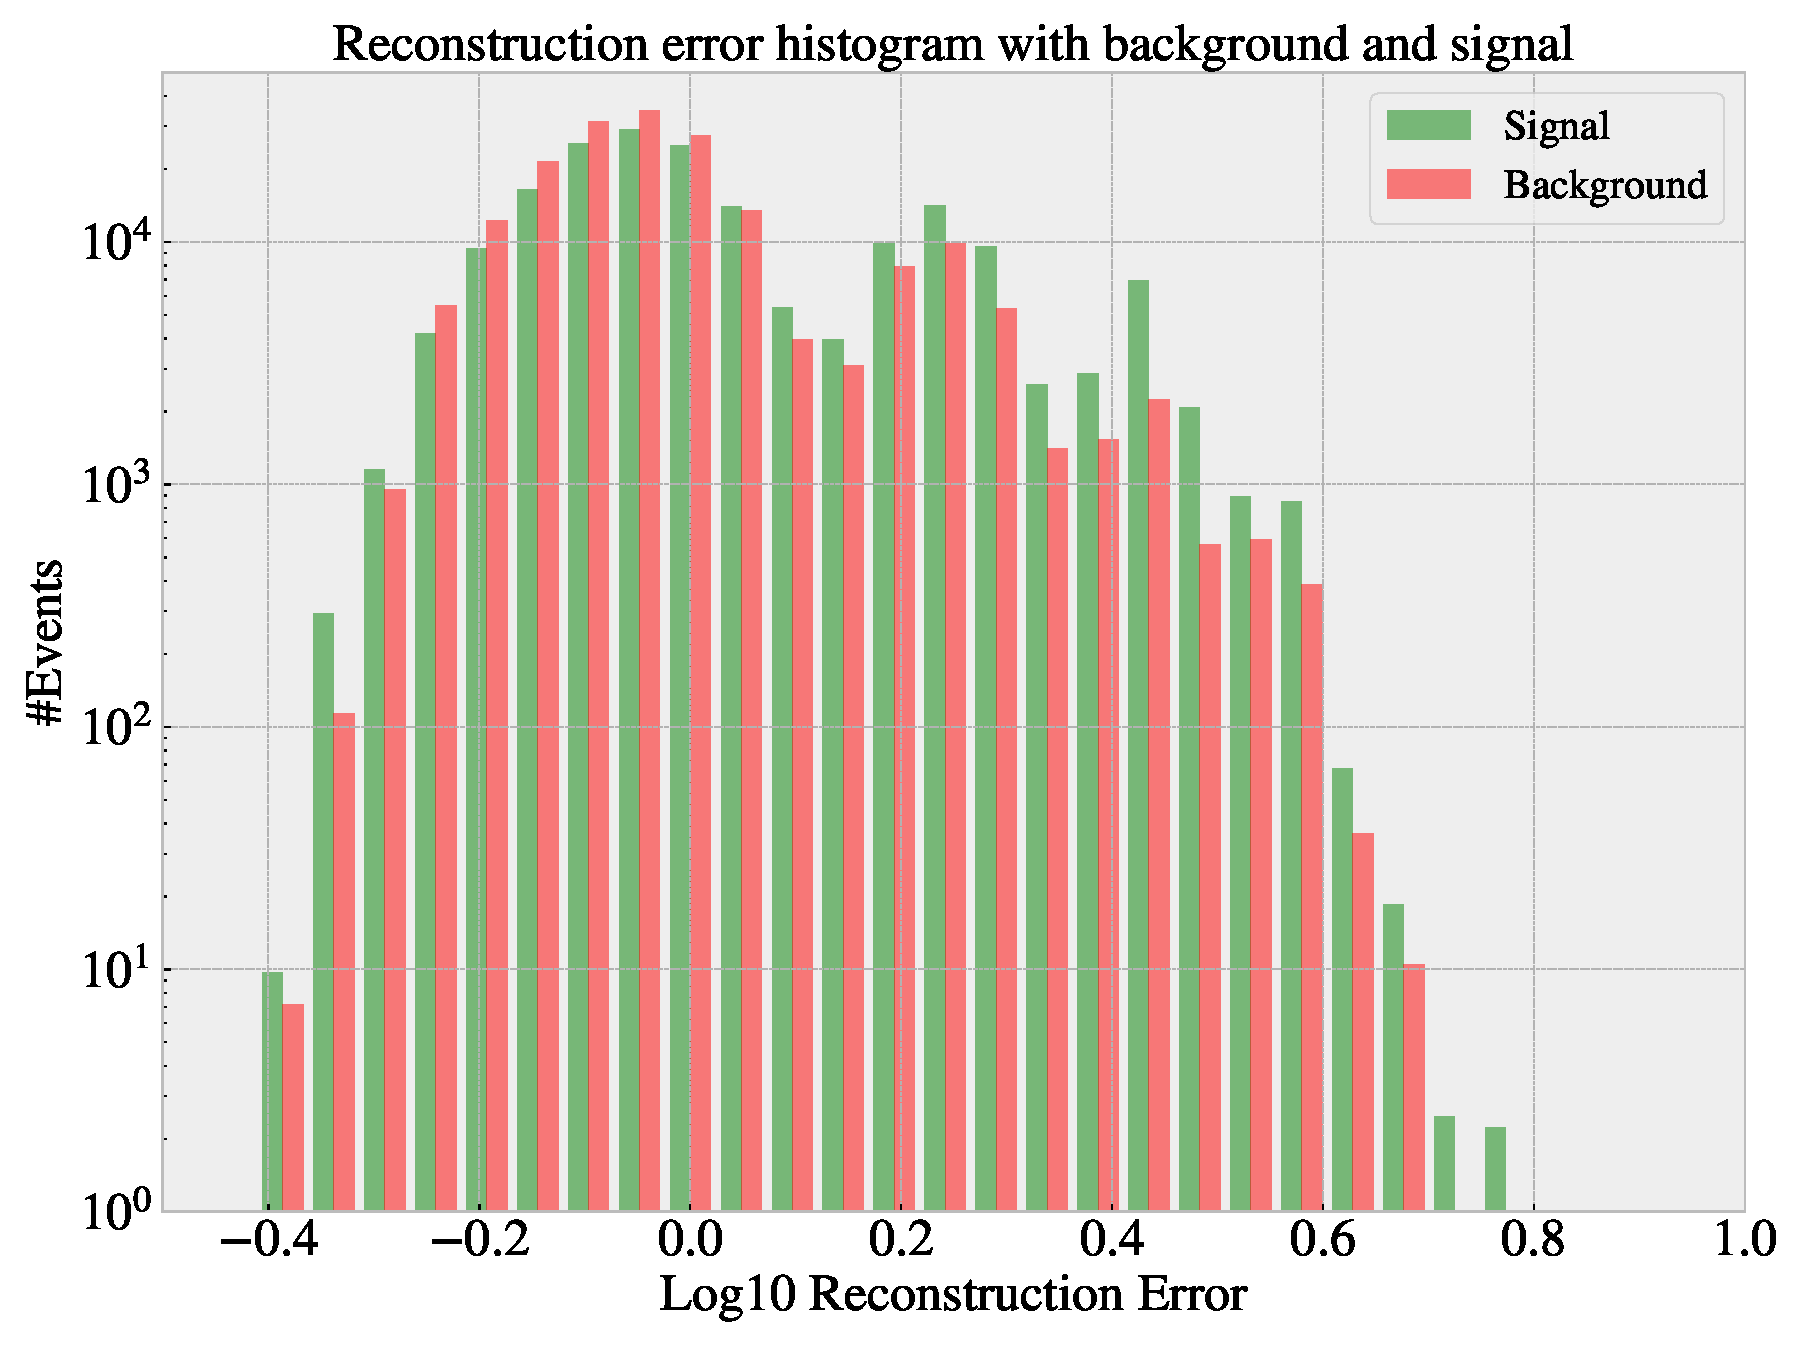
\includegraphics[width=0.46\textwidth]{figures/results/predictions/b_s_recon_big_rm3_feats.pdf}
    \caption{Reconstruction error of background MC and signal MC for big auto encoder without Graviton to dimuons.  }
    \label{fig:s_b_big_allsig_nogmumu}
\end{figure}

\begin{figure}[H]    
  \centering
         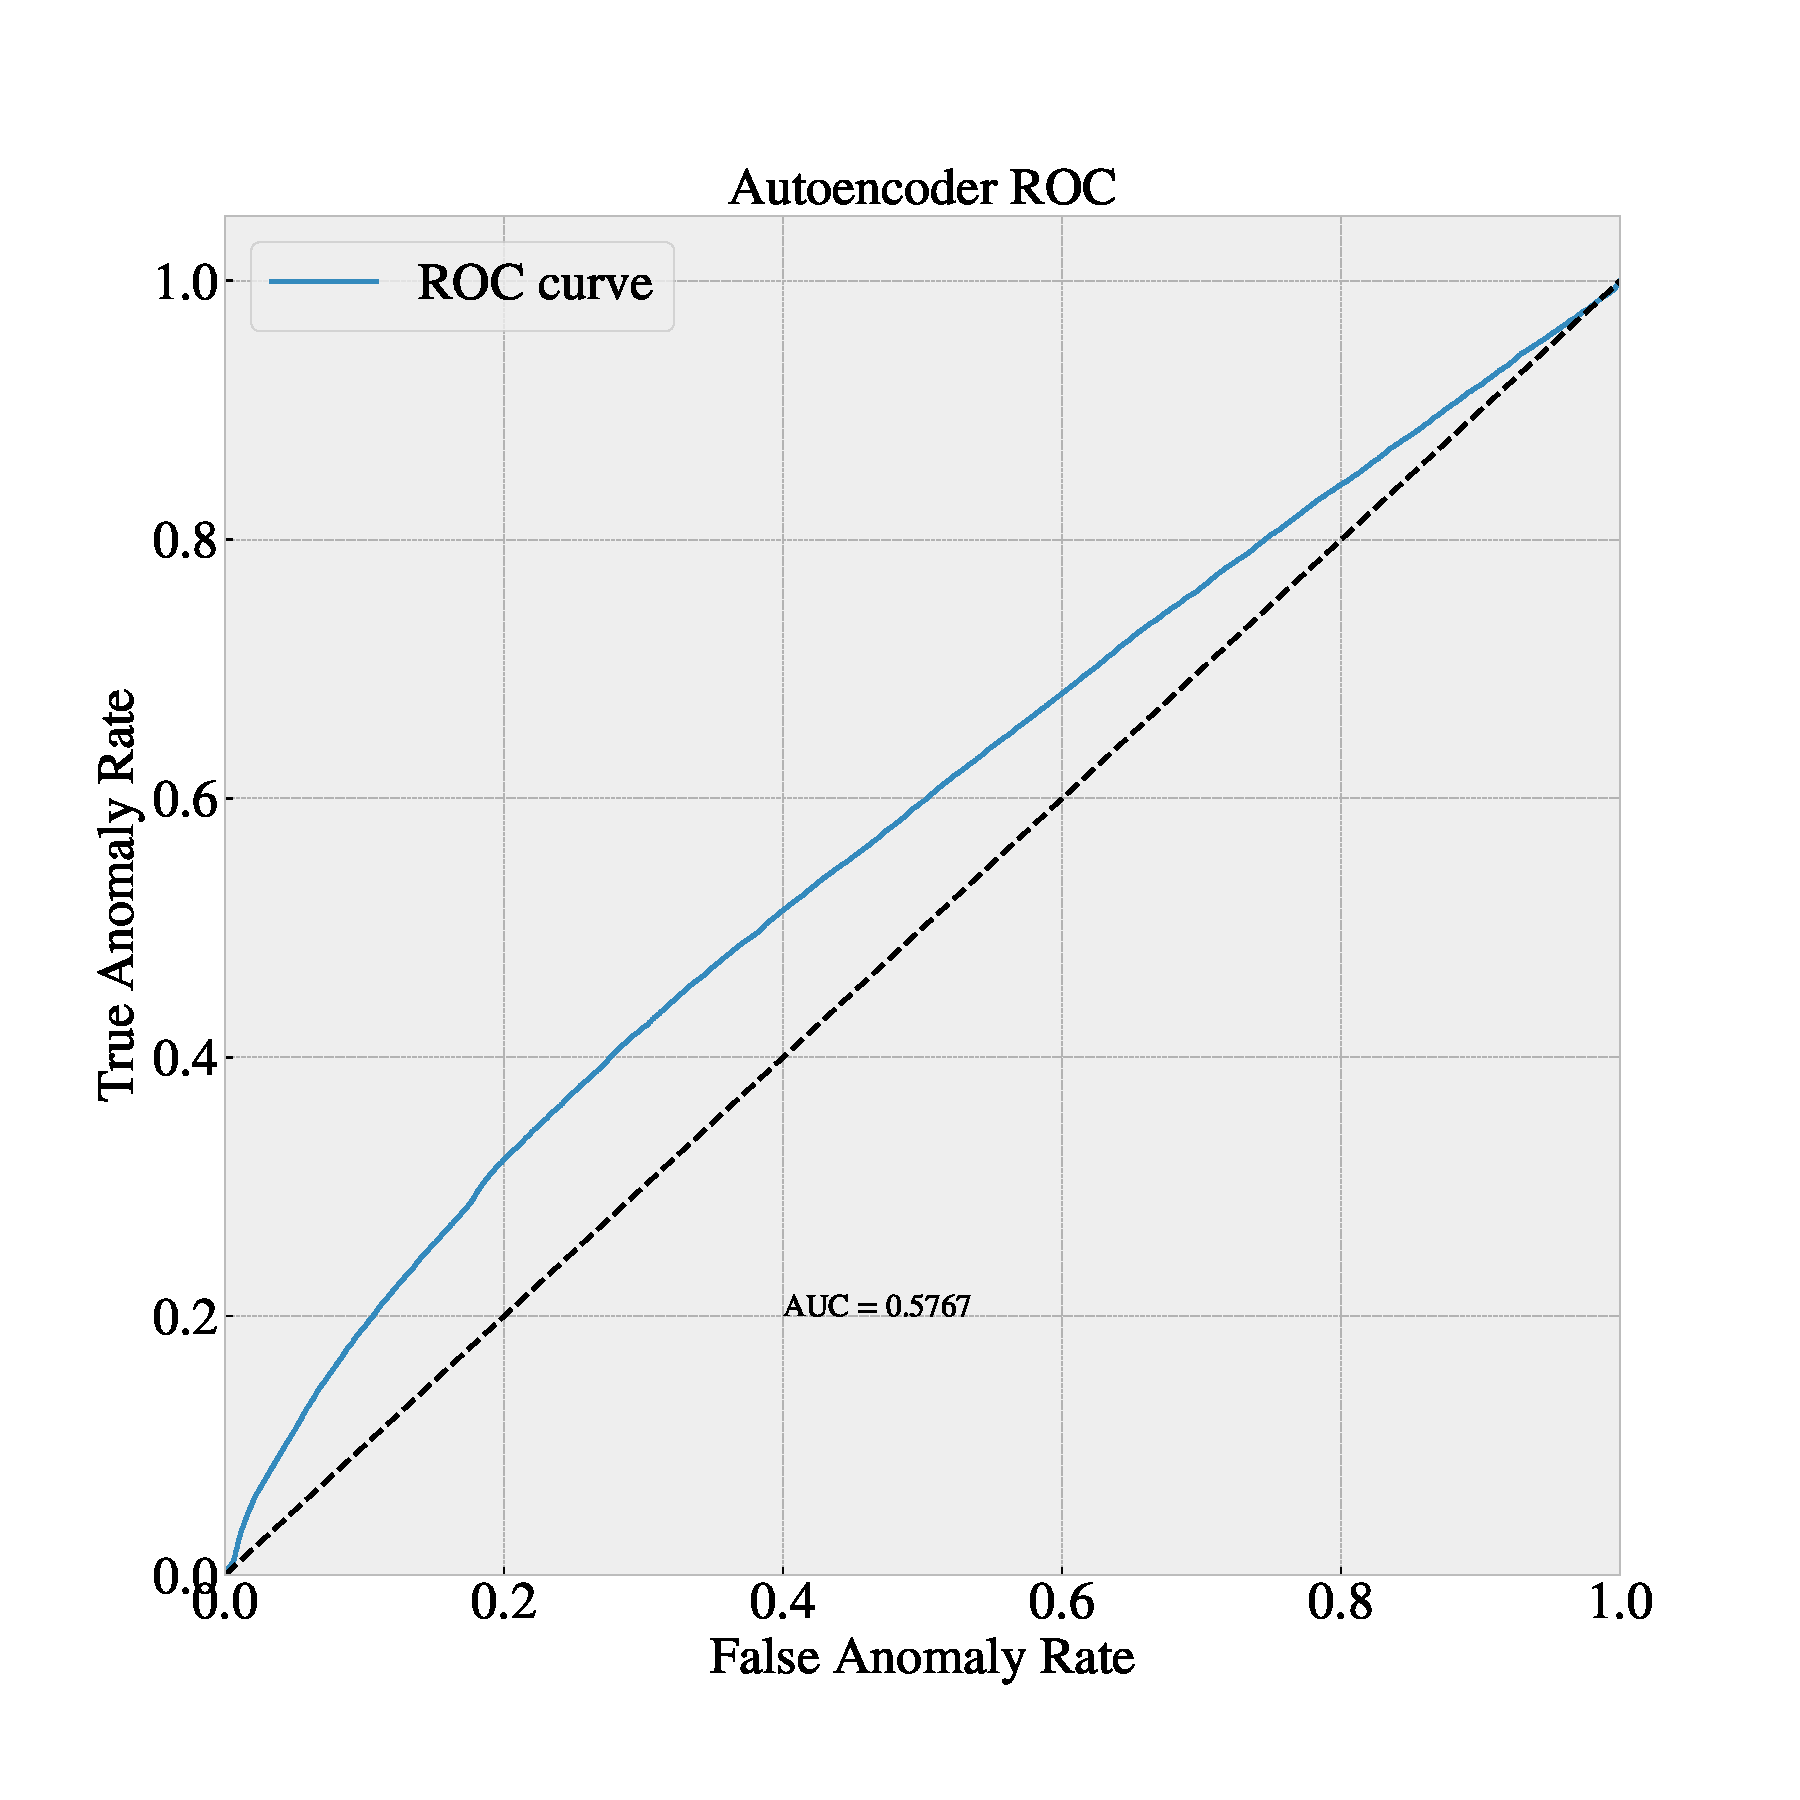
\includegraphics[width=0.46\textwidth]{figures/results/rocs/b_s_roc_curve_big_rm3feats.pdf}
         \caption{ROC curve signal MC and background MC for big auto encoder without Graviton to dimuons. }
         \label{fig:roc_sig_big_allsig_nogmumu}
\end{figure}


In figure \ref{fig:s_b_big_allsig_nogmumu} and \ref{fig:roc_sig_big_allsig_nogmumu} clearly see that the auto encoder struggles to separate background and signal MC, with a AUC score of around 0.58. This shows that for signals that are fairly similar to background MC, this model will struggle to tell them apart. There are possibilities to try to mediate this. 

\subsection{Attempts at improvement}

One such method is altering the architecture of the auto encoder. To compare this architecture I created a smaller auto encoder, shown in figure \ref{fig:small_ae_plot}.

\begin{figure}[H]
    \centering
    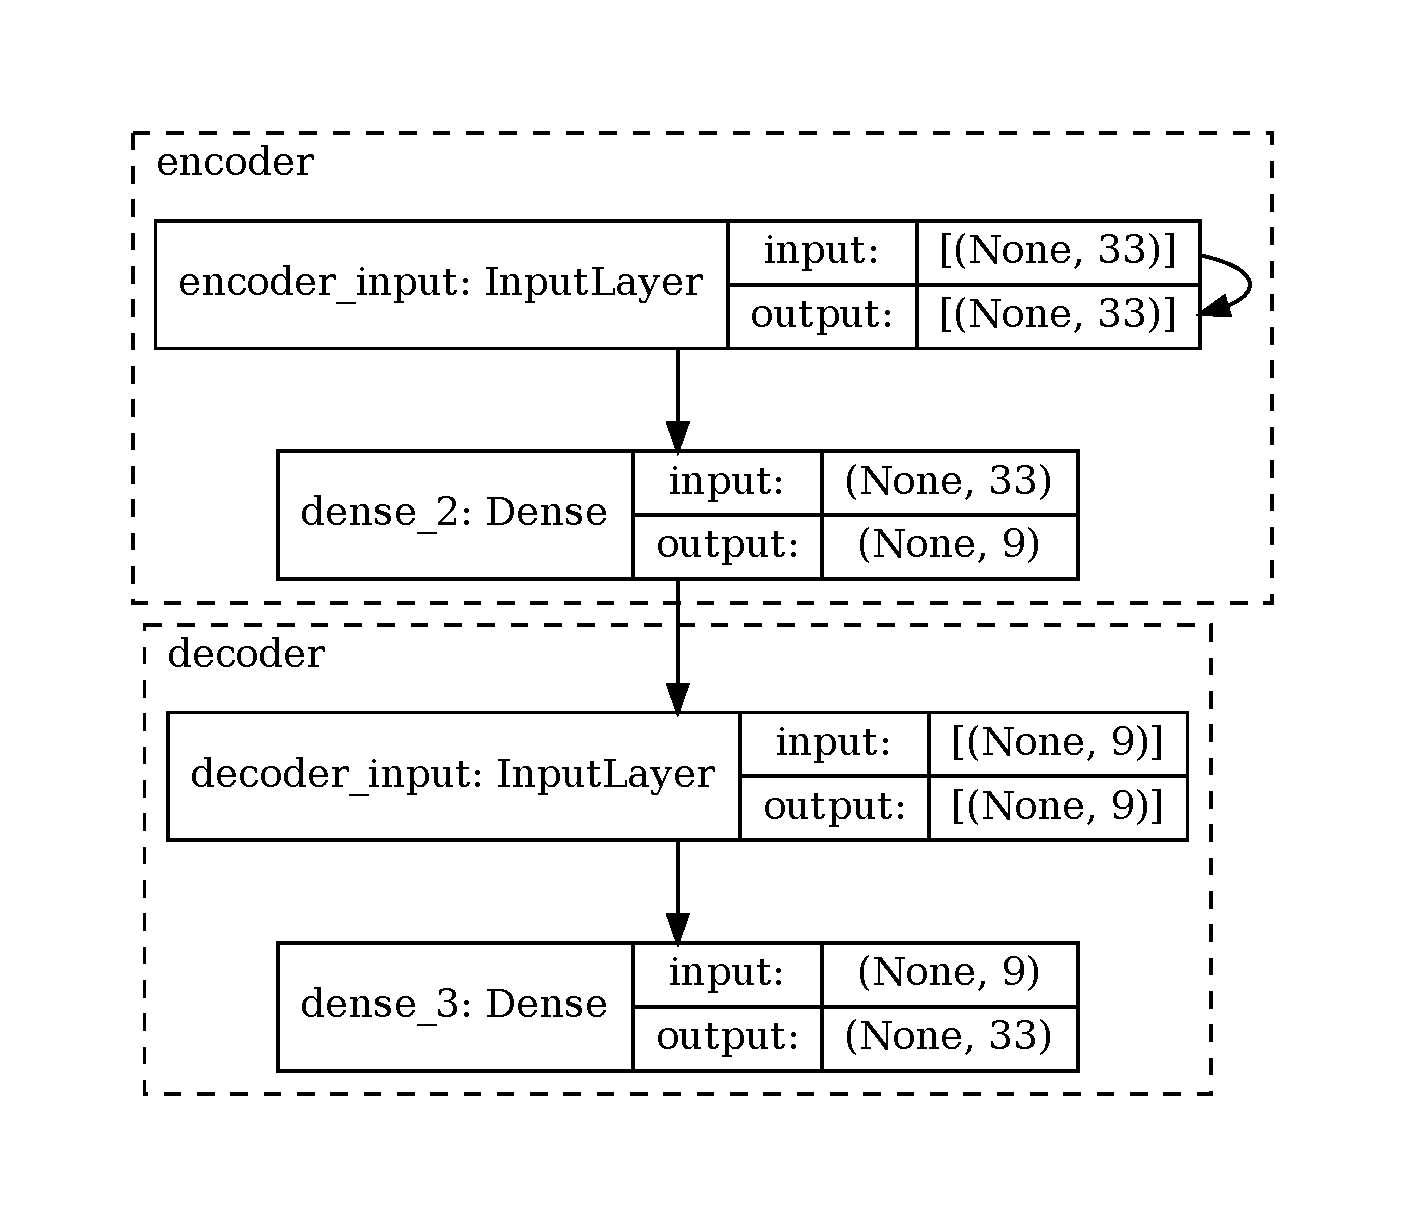
\includegraphics[width=0.46\textwidth]{figures/results/models/ae_model_plot_small.pdf}
    \caption{Smaller auto encoder architecture after grid search. }
    \label{fig:small_ae_plot}
\end{figure}

The hyper parameters used for this model was a learning rate of 0.9, 24 nodes in the latent space, the activation function for the latent space was tanh, the activation function for the output was linear, the kernel regularization was 0.05 and the activation regularization was 0.01. The model was trained for 6 epochs.


\begin{figure}[H]
     \centering
         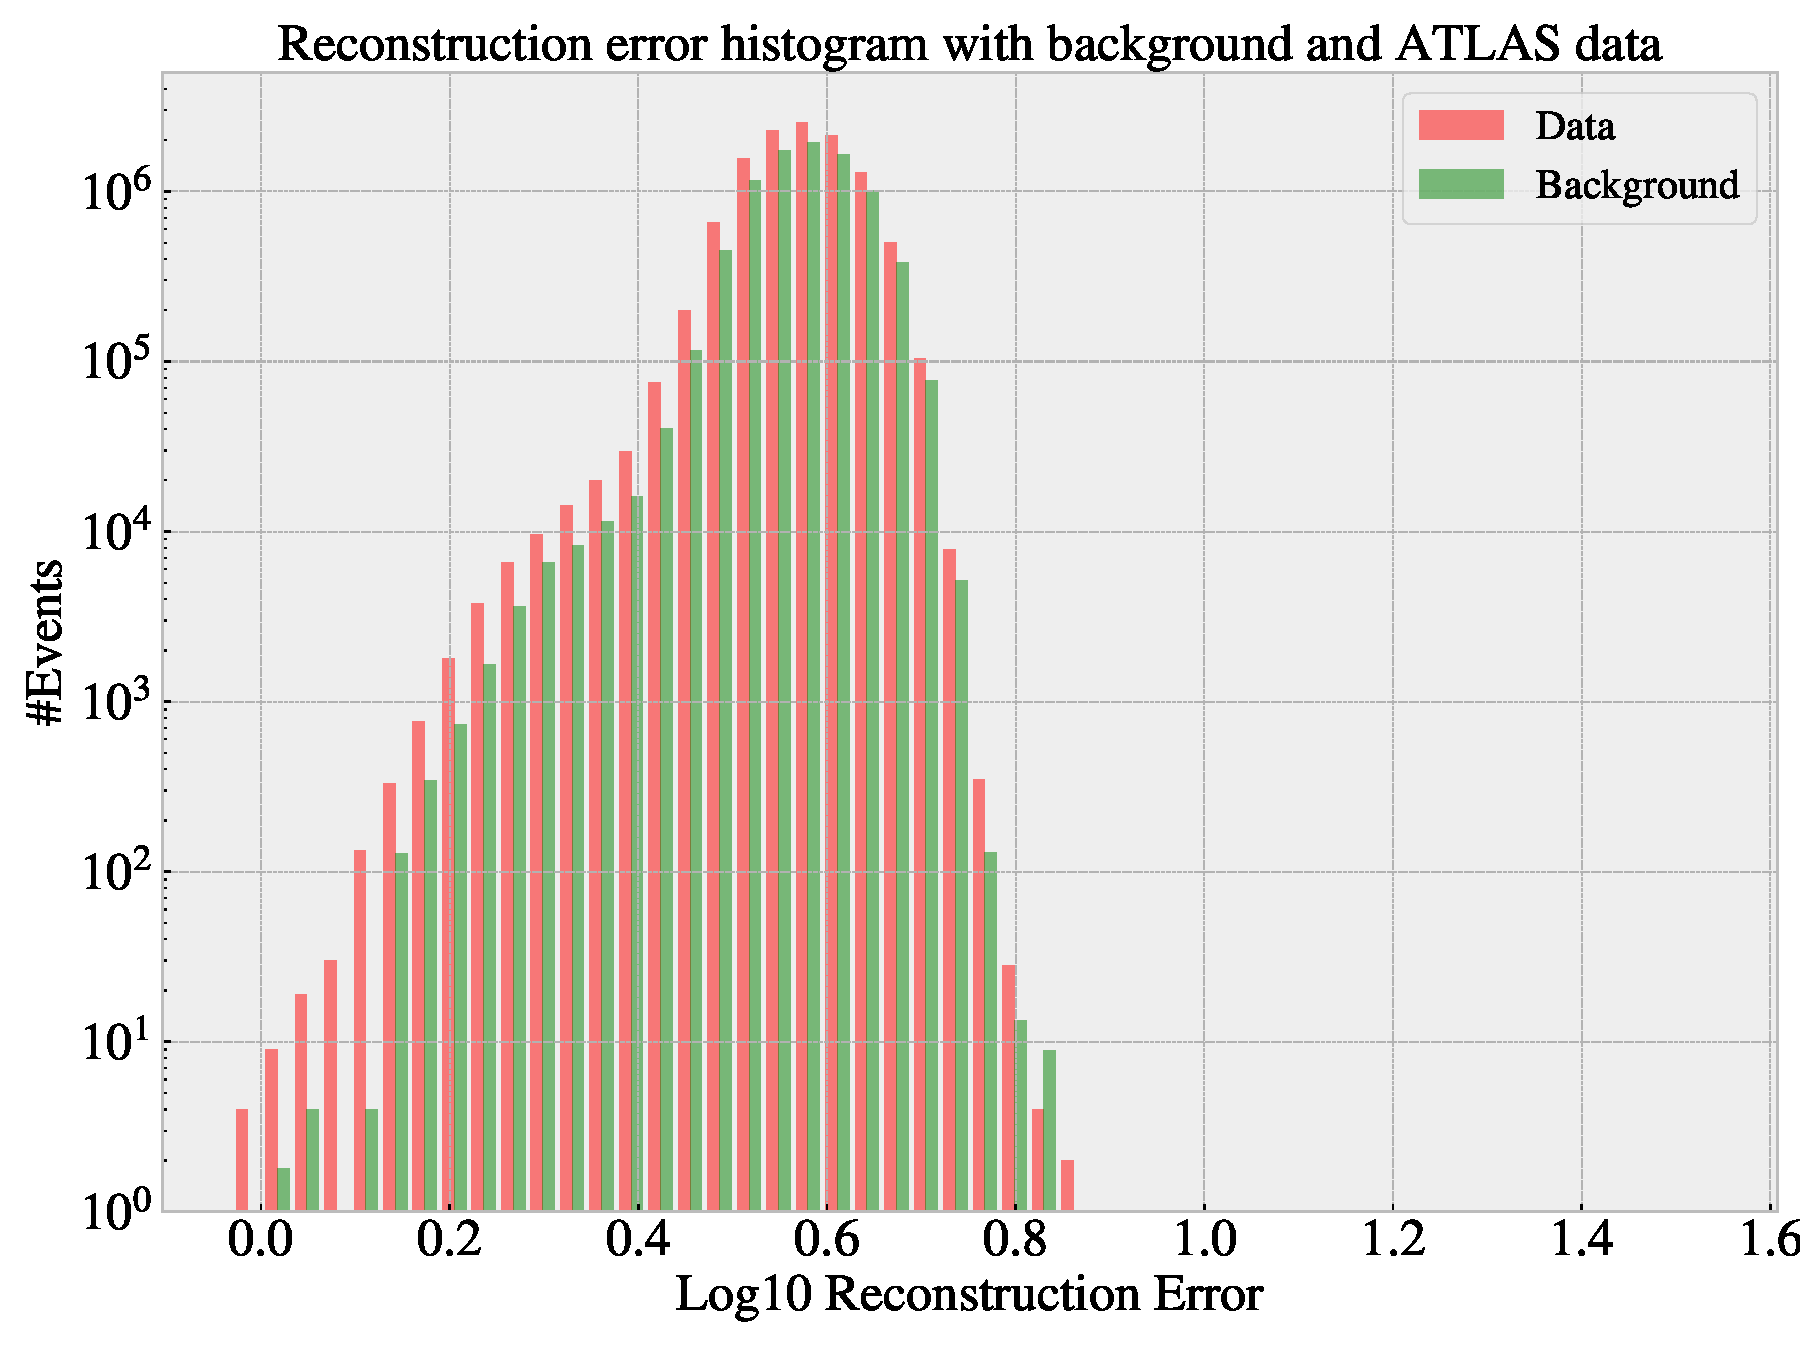
\includegraphics[width=0.46\textwidth]{figures/results/predictions/b_data_recon_small_rm3_feats_nogmumu.pdf}
         \caption{Histogram showing reconstruction error for ATLAS data and background MC for small auto encoder. }
     \label{fig:data_b_small_pred}
\end{figure}

Using the architecture in figure \ref{fig:small_ae_plot} I get a good overlap of ATLAS data and background MC, with a center of about 4 MSE reconstruction error. 

\begin{figure}[H]    
 \centering
    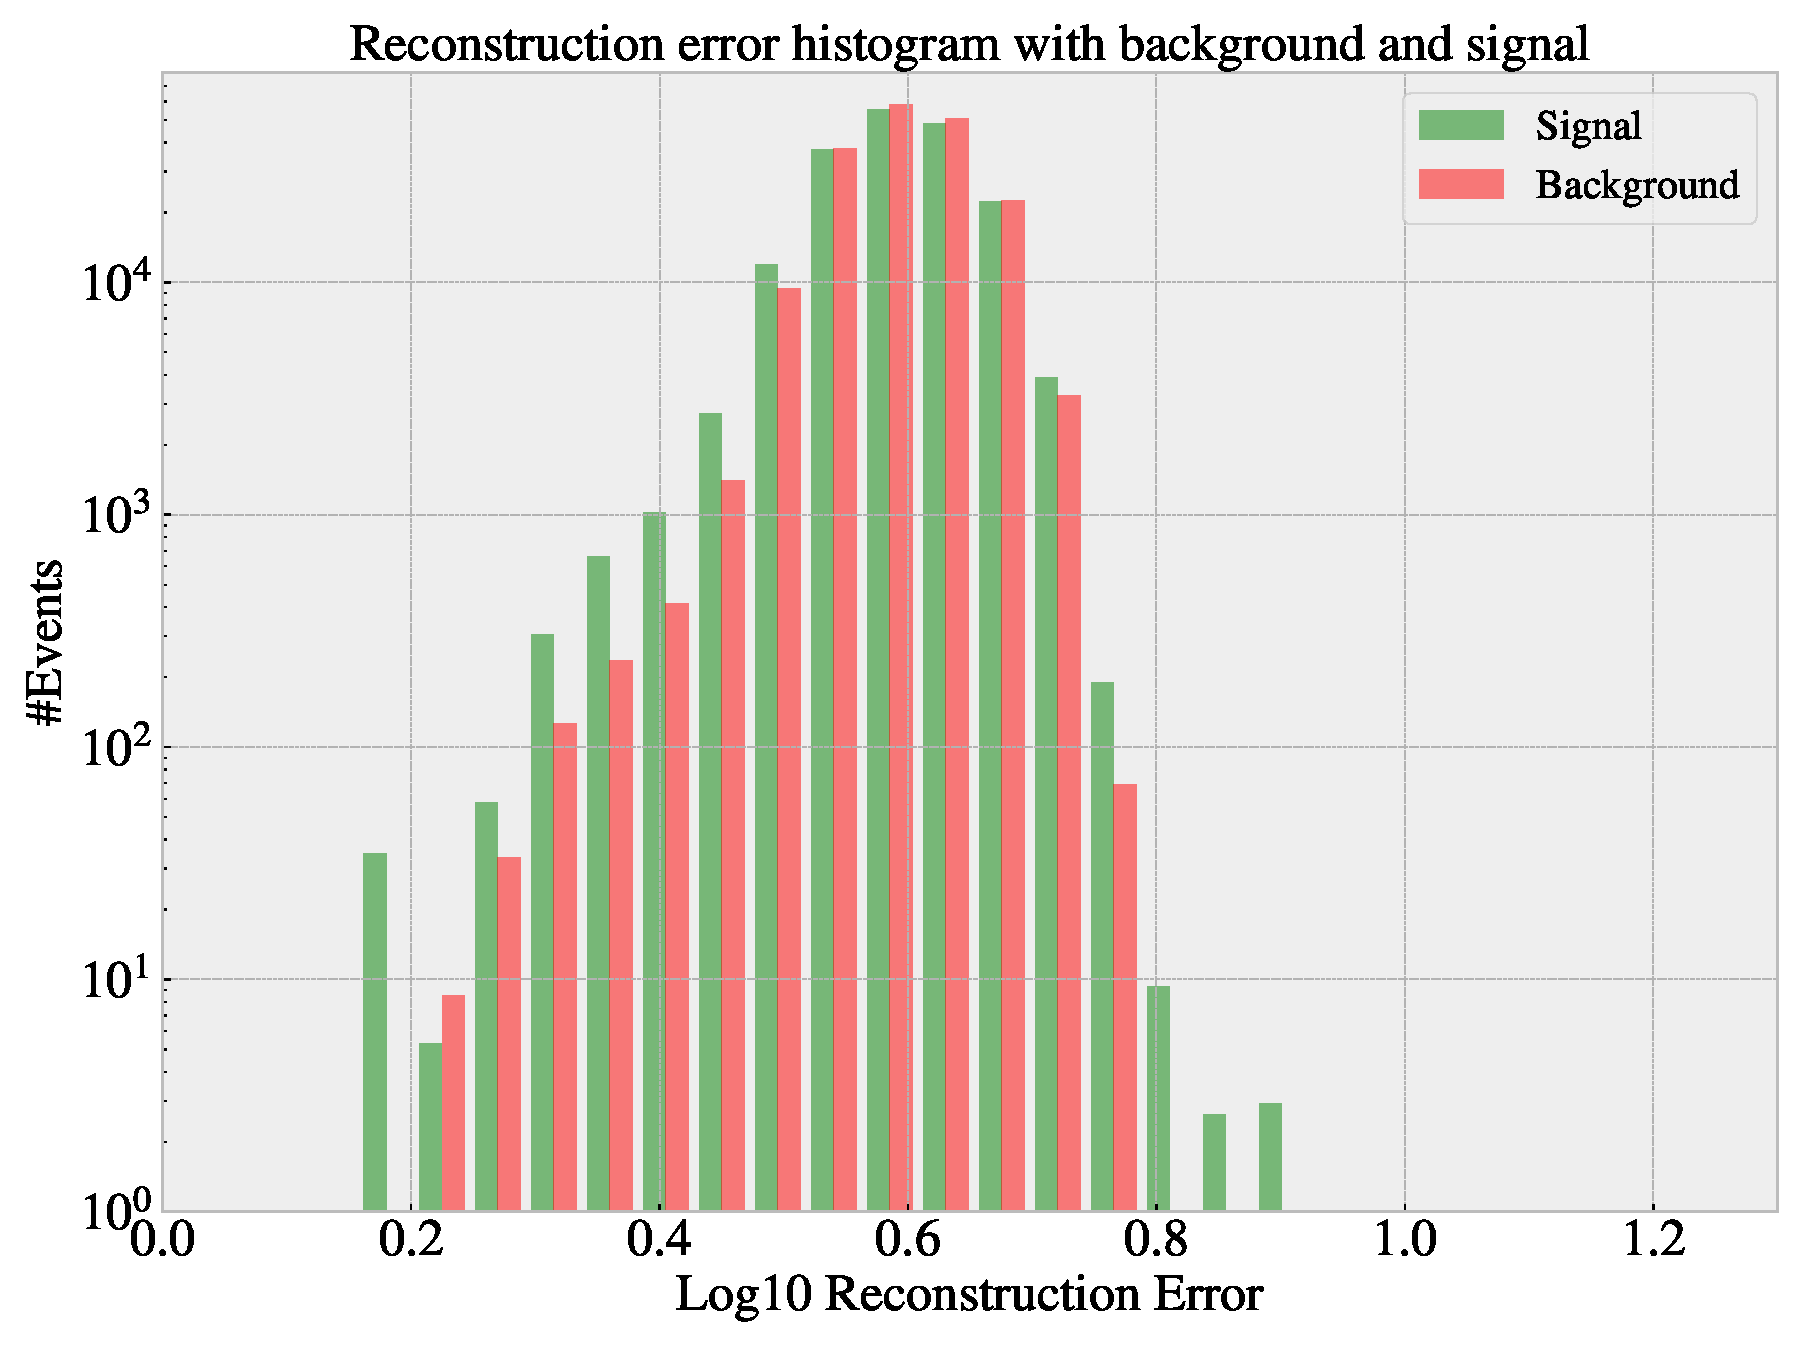
\includegraphics[width=0.46\textwidth]{figures/results/predictions/b_s_recon_small_rm3_feats_nogmumu_nolog.pdf}
    \caption{Reconstruction error of background MC and signal MC for small auto encoder. }
    \label{fig:s_b_small_pred_}   
  
\end{figure}

\begin{figure}[H]    
  \centering
         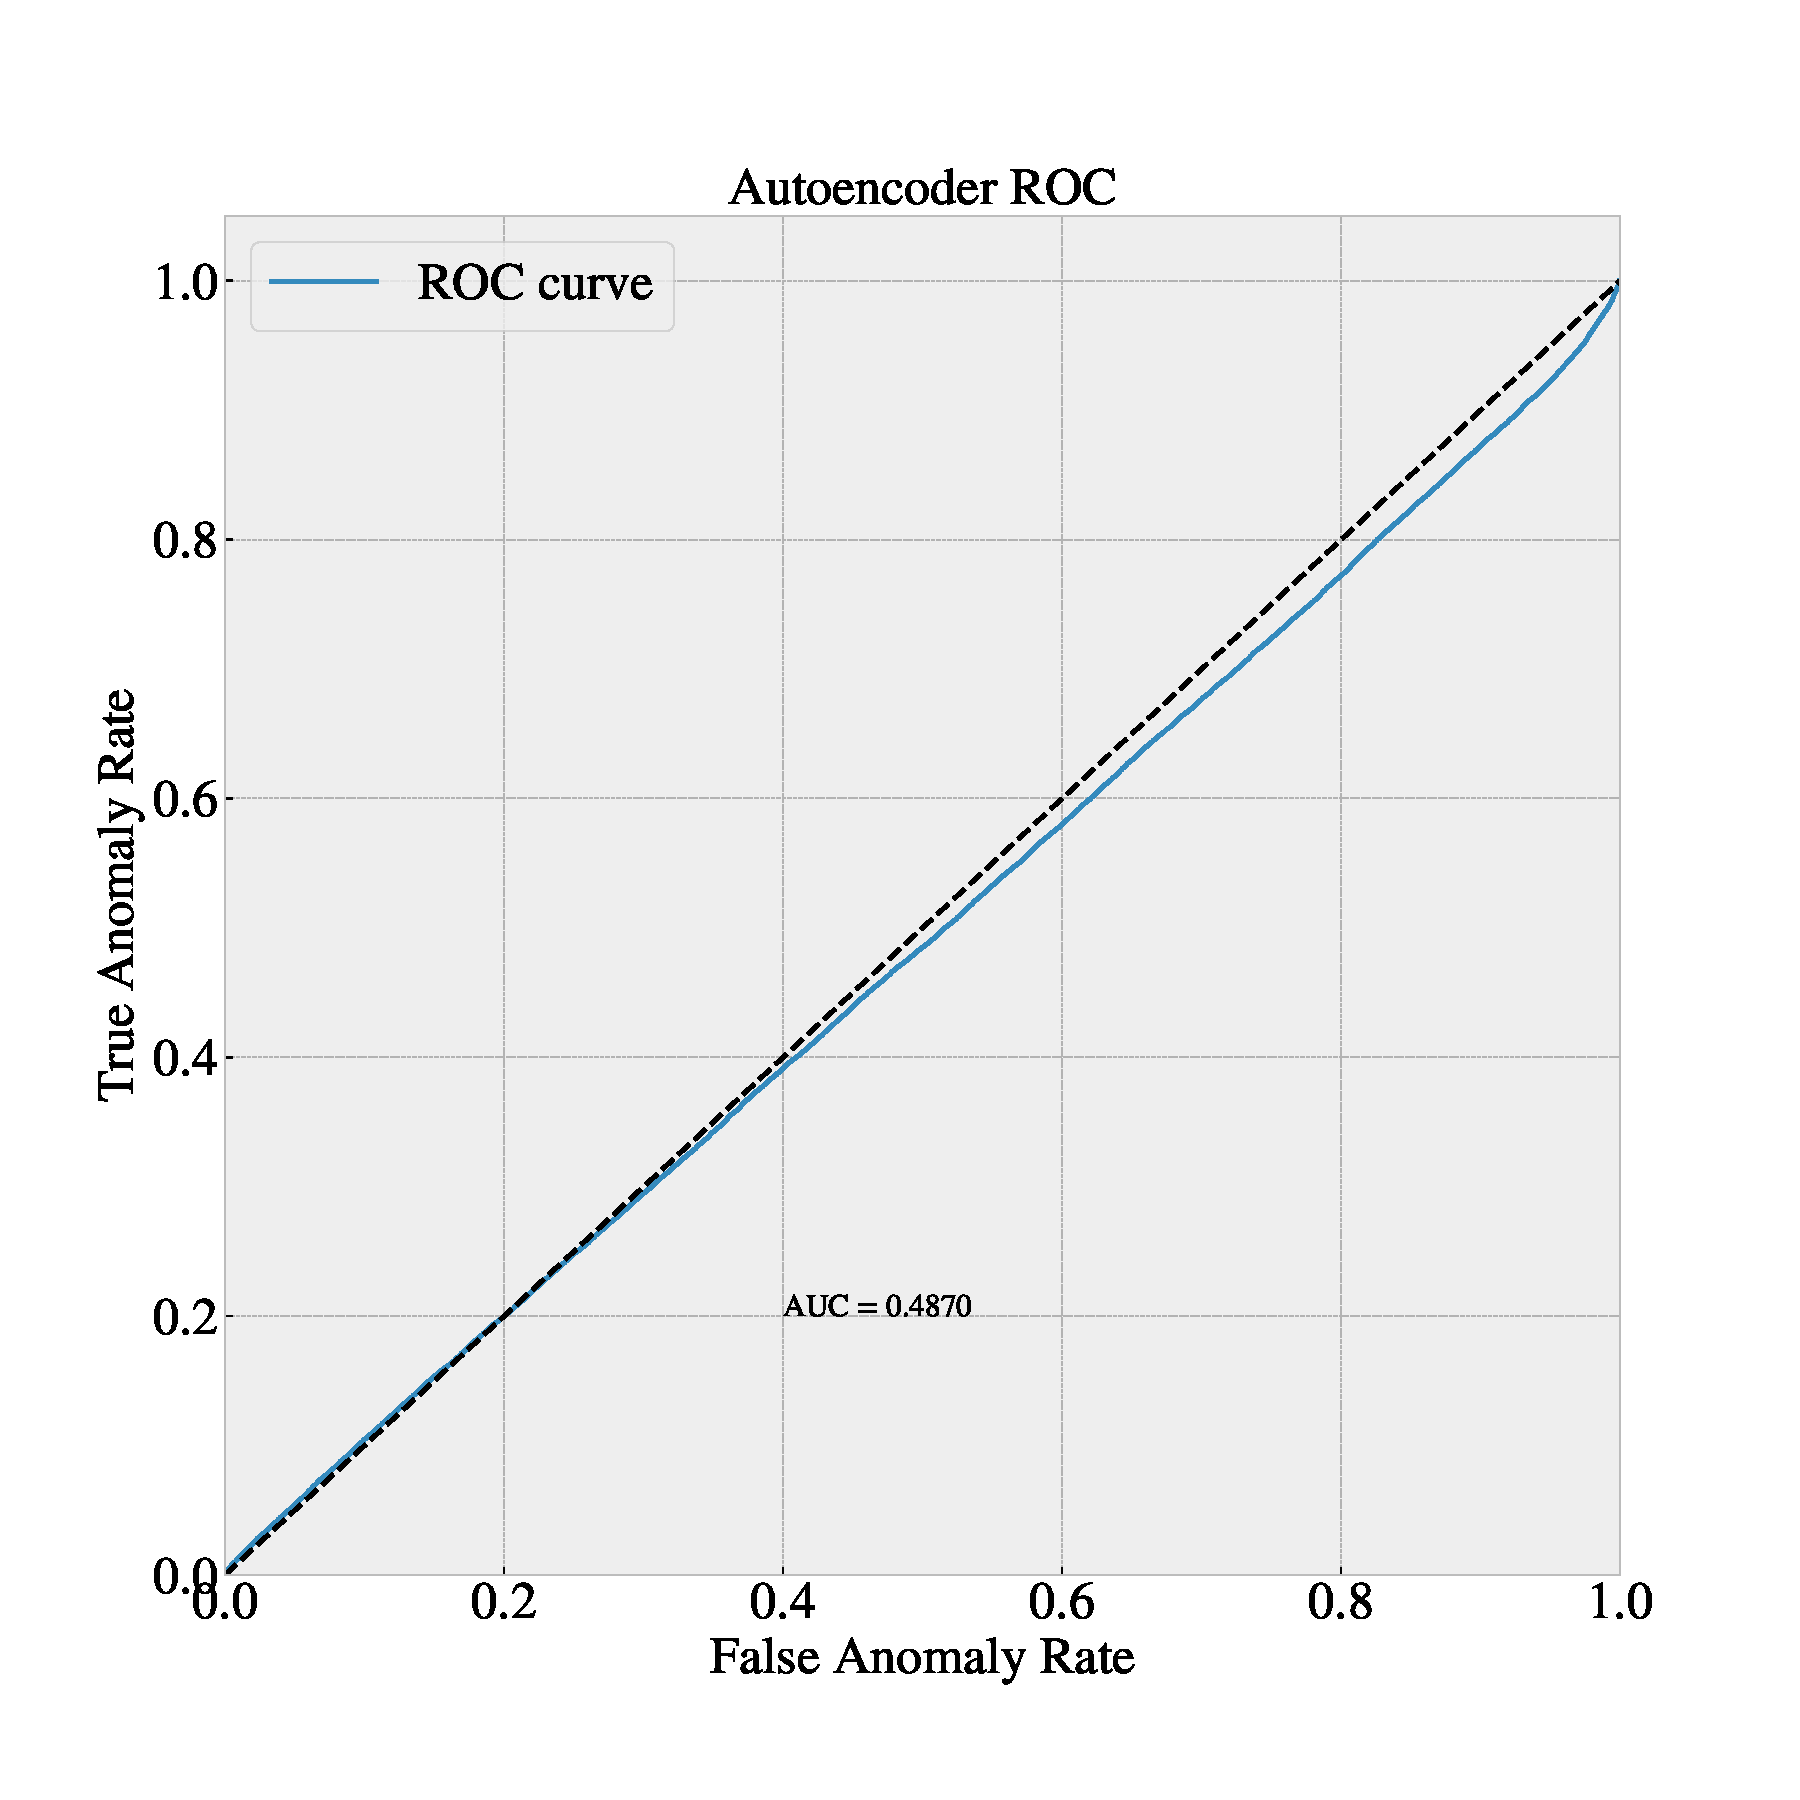
\includegraphics[width=0.46\textwidth]{figures/results/rocs/b_s_roc_curve_small_nogmumu.pdf}
         \caption{ROC curve signal MC and background MC for small auto encoder}
         \label{fig:s_b_small_roc}  
  
\end{figure}


As shown in figure \ref{fig:s_b_small_pred_} and \ref{fig:s_b_small_roc} we observe that even though this model gets a good overlap, it struggles even further than the big auto encoder, having an AUC score of only 0.48 which is only slightly better than guessing. This could mean that such a simple model needs more complexity in terms of layers and node reduction per layer to be able to learn how to separate.\par 
Another idea is removing low level features that are fairly similar for background and signal MC. From testing it was found that even with as low as 13 features, the output from the algorithm only improved slightly.

\begin{figure}[H]    
  \centering
         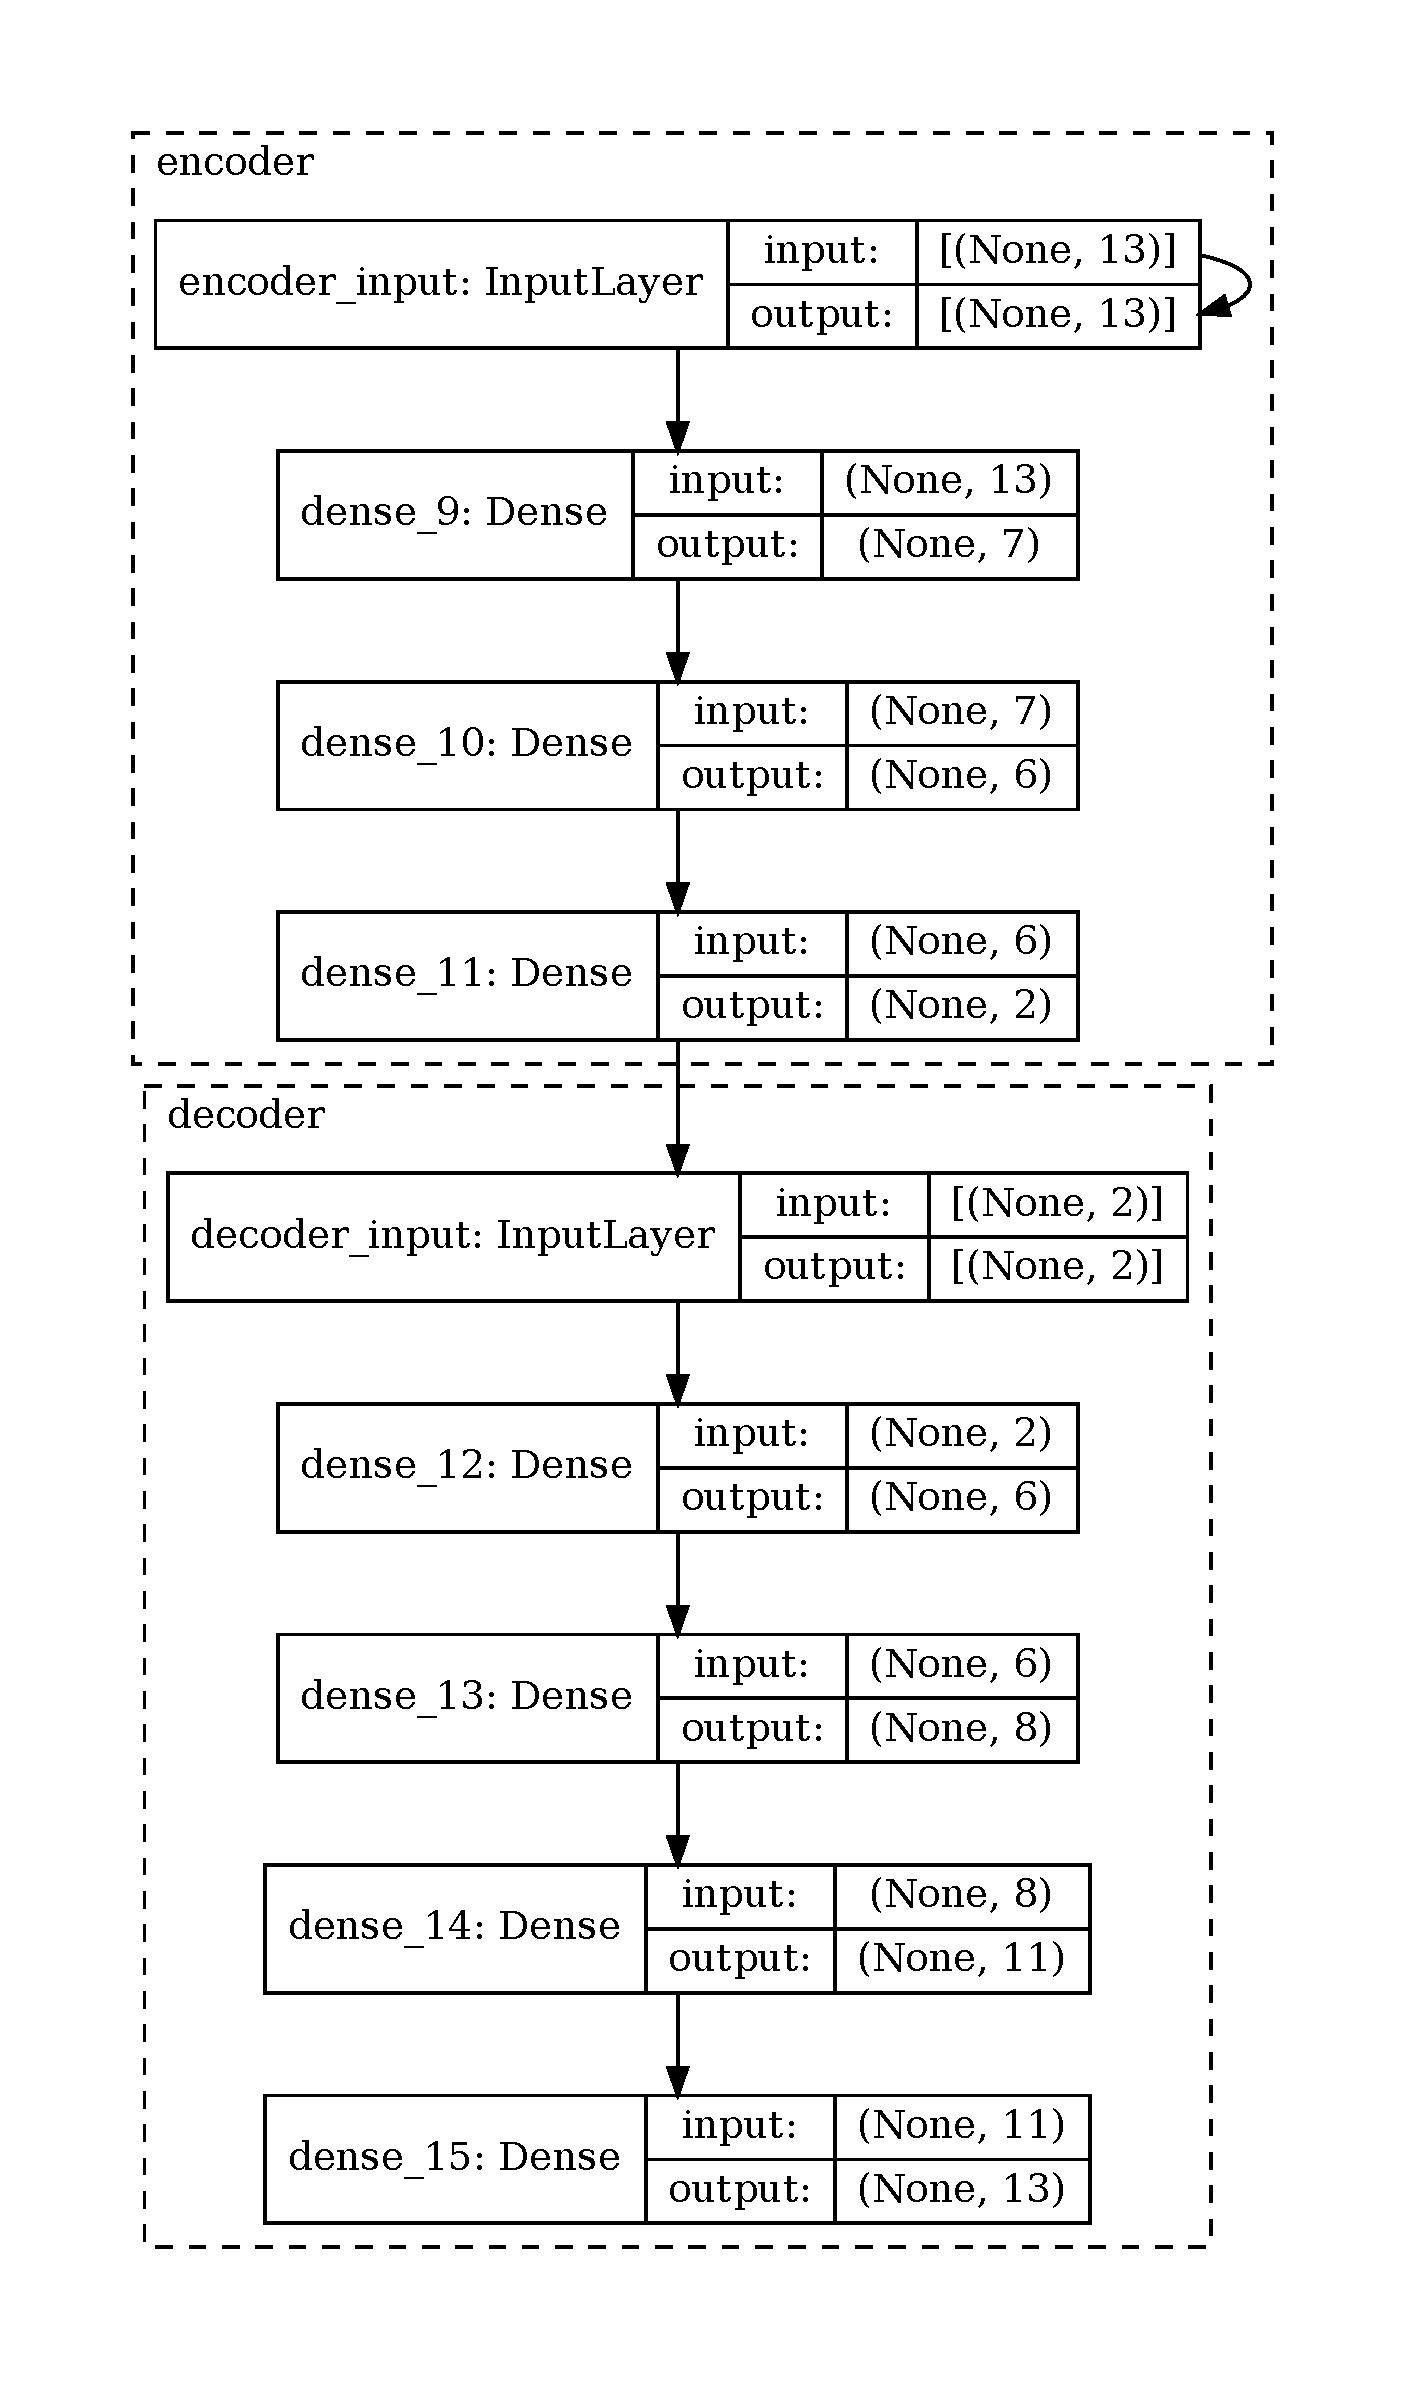
\includegraphics[width=0.46\textwidth]{figures/results/models/ae_model_plot_13feats_big.pdf}
         \caption{Auto encoder architecture found by hyper parameter search with 13 features in the input.}
         \label{fig:ae_13feats_big}  
  
\end{figure}

In figure \ref{fig:ae_13feats_big} we have the tuned auto encoder architecture based on a hyper parameter search for 13 feature dataset. The hyper parameters were as follows. The encoder had leakyrelu, linear, leakyrelu as activation functions. The latent space had 2 nodes and linear as activation function. The decoder had leakyrelu, tanh, relu and linear as activation functions. The kernel regularization was 0.5, the activation regularization was 0.5, the leakyrelu alpha parameter was 0.1 and the learning rate was 0.0015. The model was trained with 5 epochs.

\begin{figure}[H]
     \centering
         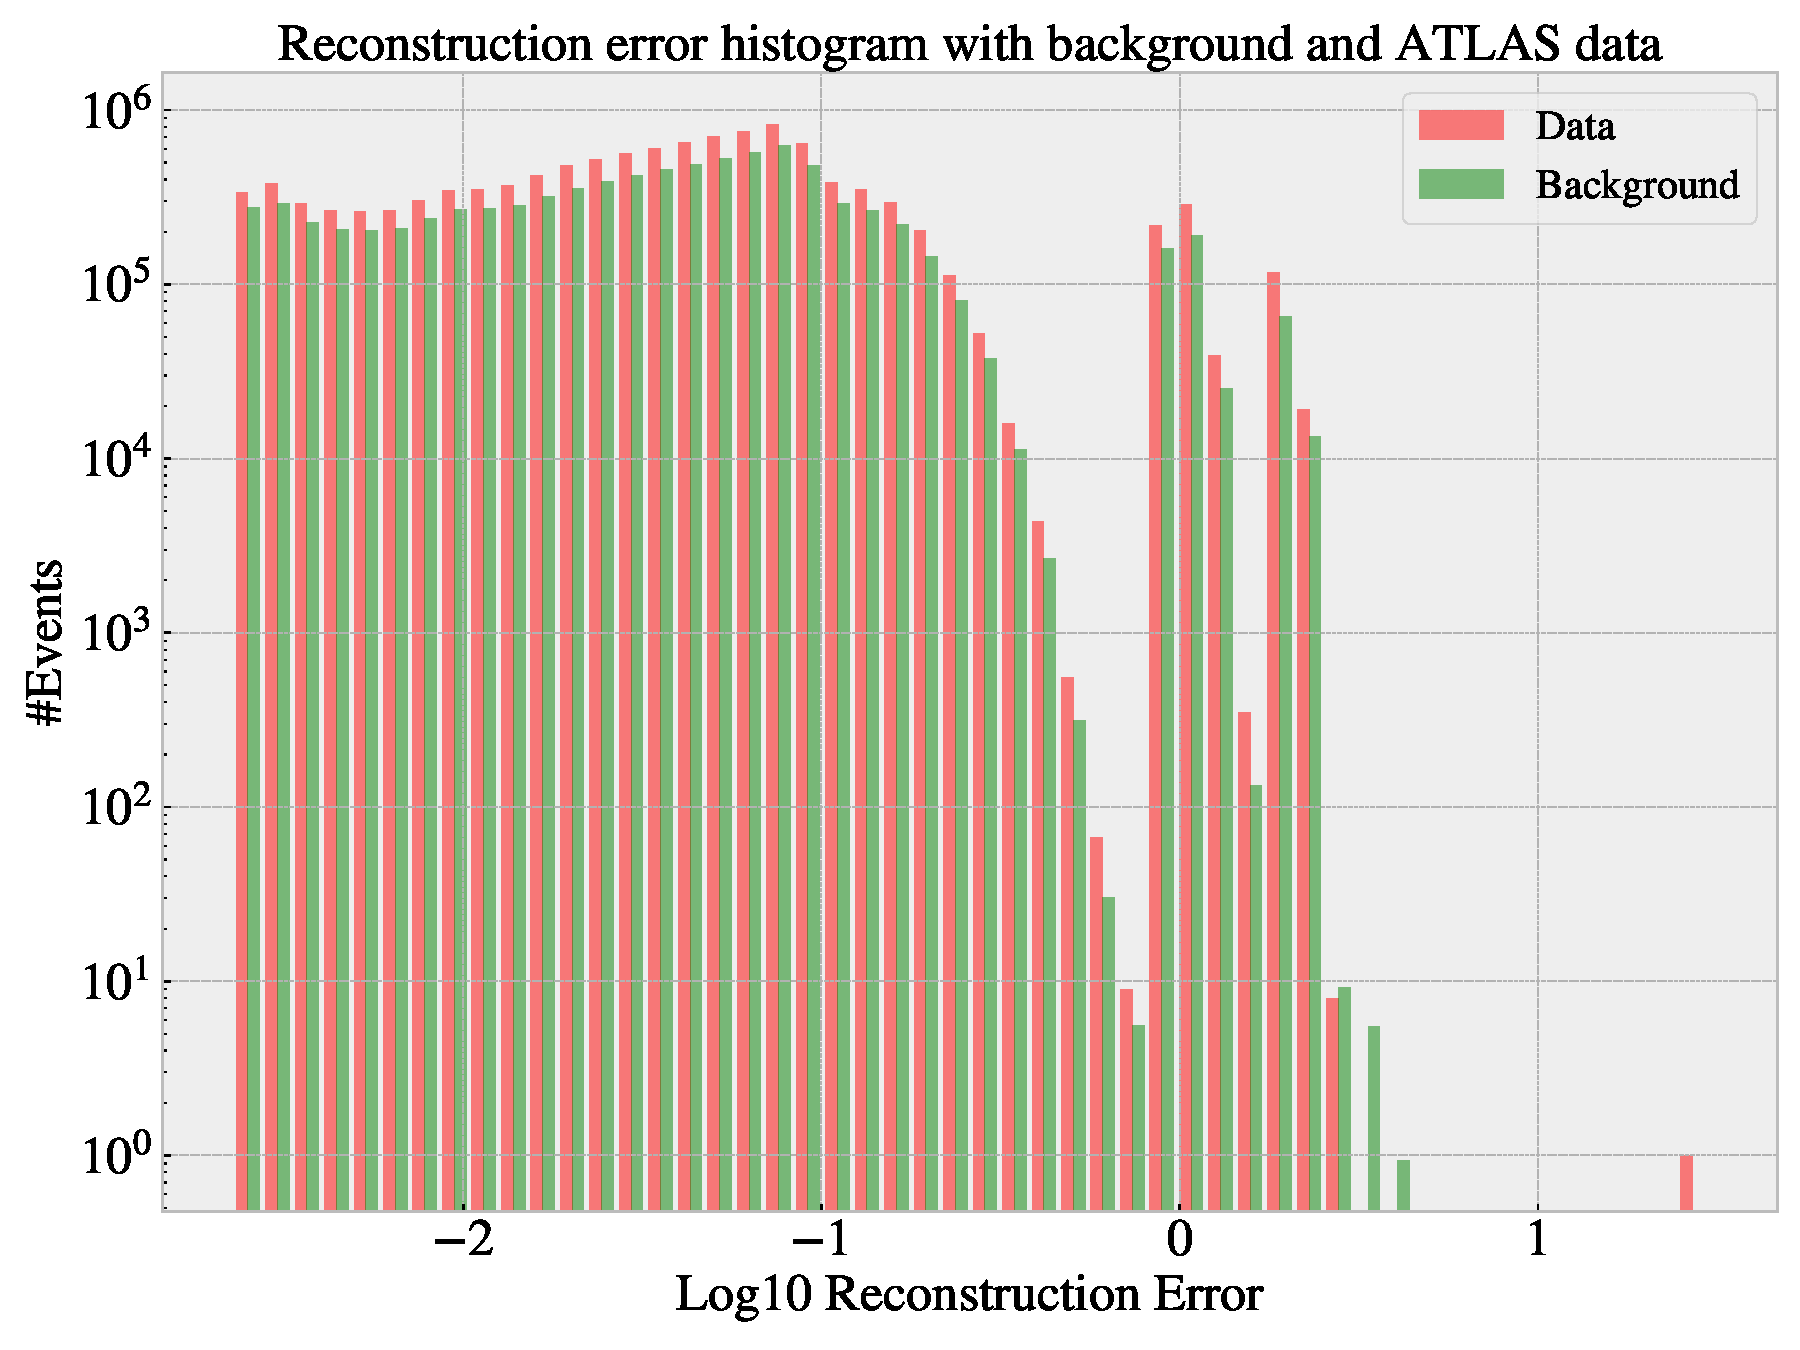
\includegraphics[width=0.46\textwidth]{figures/results/predictions/b_data_recon_big_rm3_feats_rmmanyfeats_loglog.pdf}
         \caption{Histogram showing reconstruction error for ATLAS data and background MC for big auto encoder using only 13 features.}
     \label{fig:data_b_big_pred_13feats}
\end{figure}

In figure \ref{fig:data_b_big_pred_13feats} we observe that the reconstruction error of ATLAS data and background MC have fairly good overlap. As expected the reconstruction distribution is centered at a much lower value than for the larger data sets, as there are a lot fewer features to reconstruct. 

\begin{figure}[H]
    \centering
    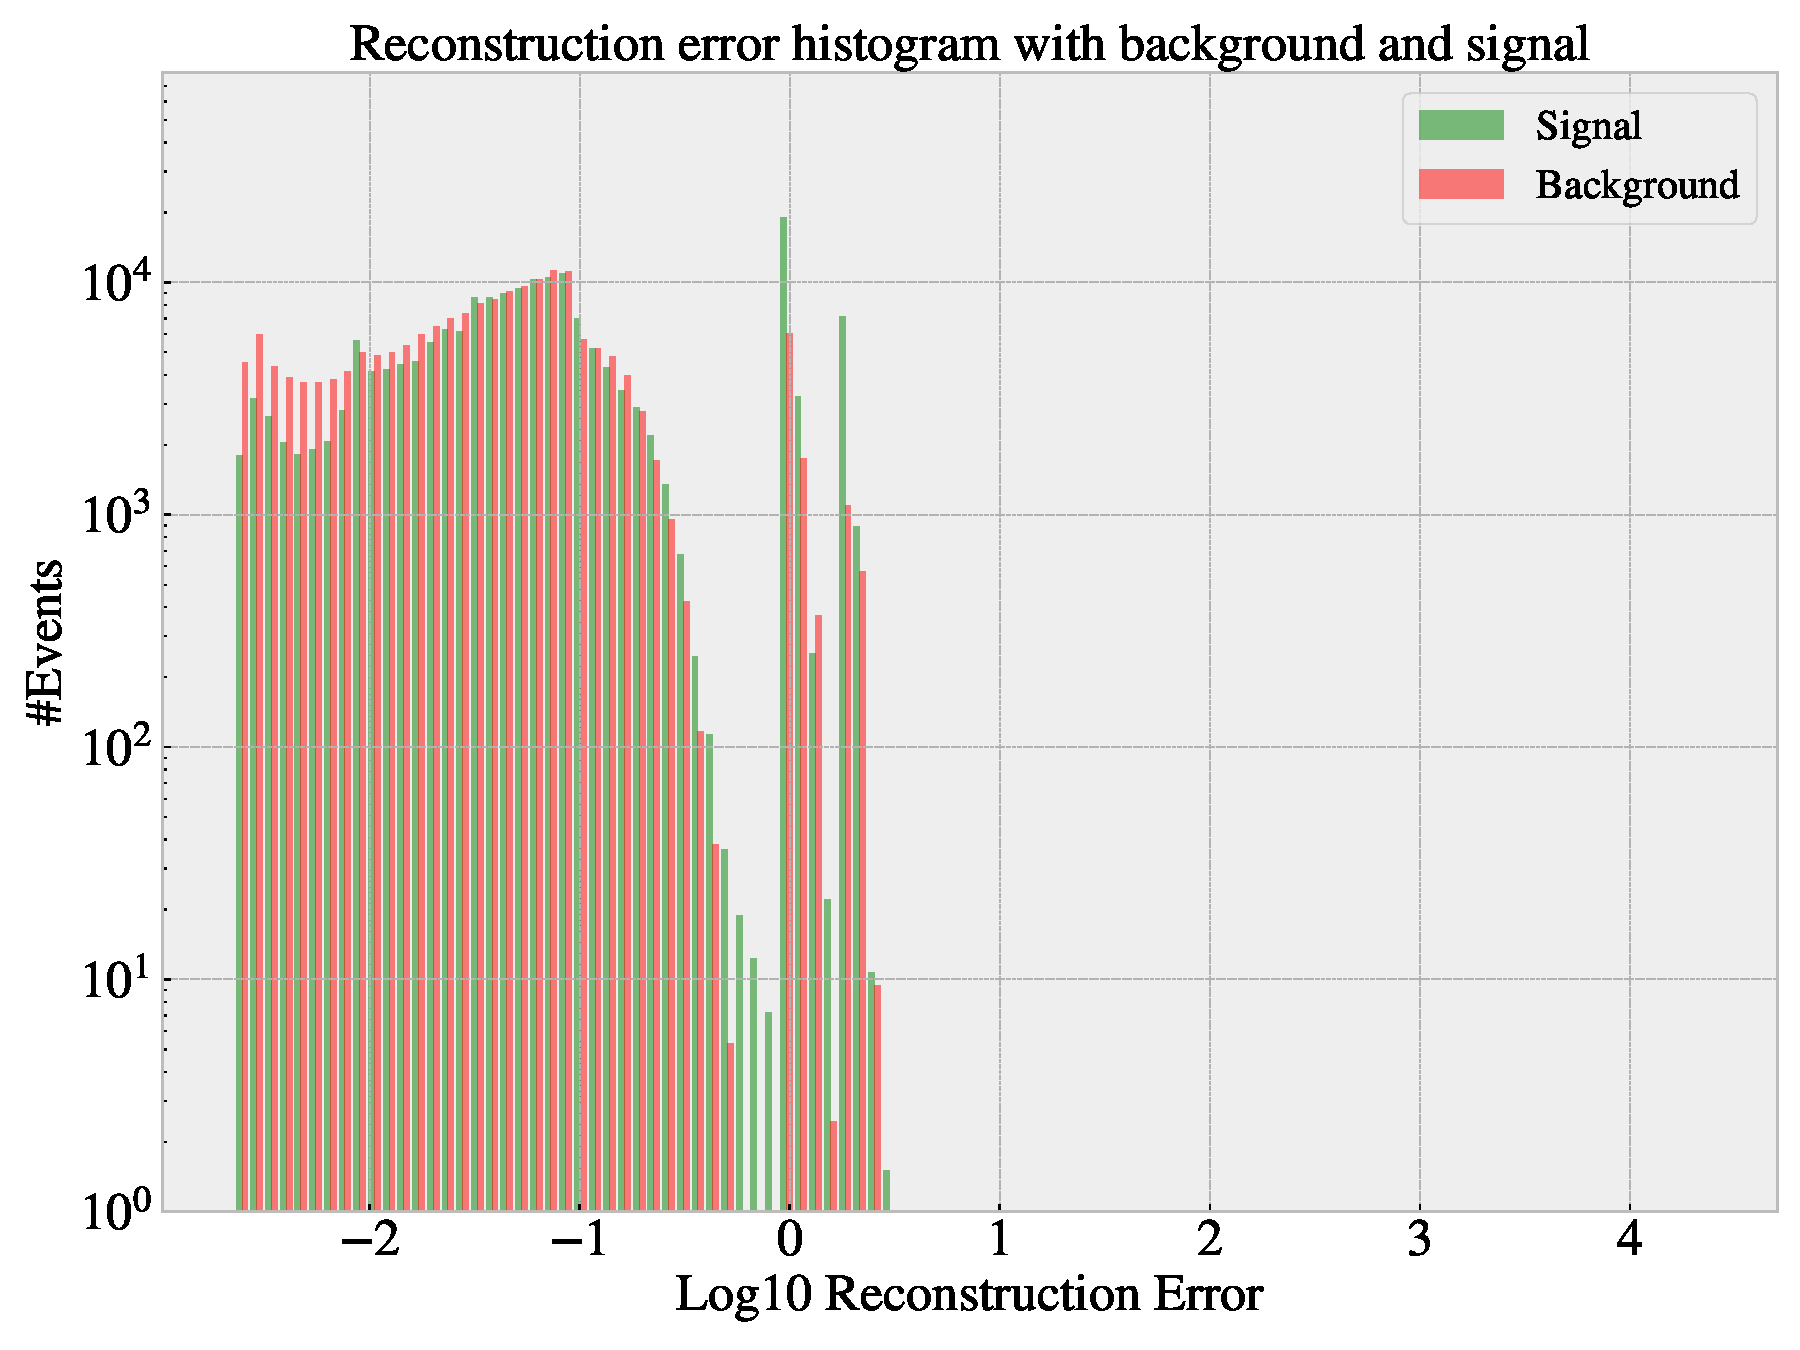
\includegraphics[width=0.46\textwidth]{figures/results/predictions/b_s_recon_big_rm3_feats_rmmanyfeats_loglog.pdf}
    \caption{Reconstruction error of background MC and signal MC for big auto encoder using only 13 features. }
    \label{fig:roc_sig_big_13feats}
\end{figure}

\begin{figure}[H]
    \centering
         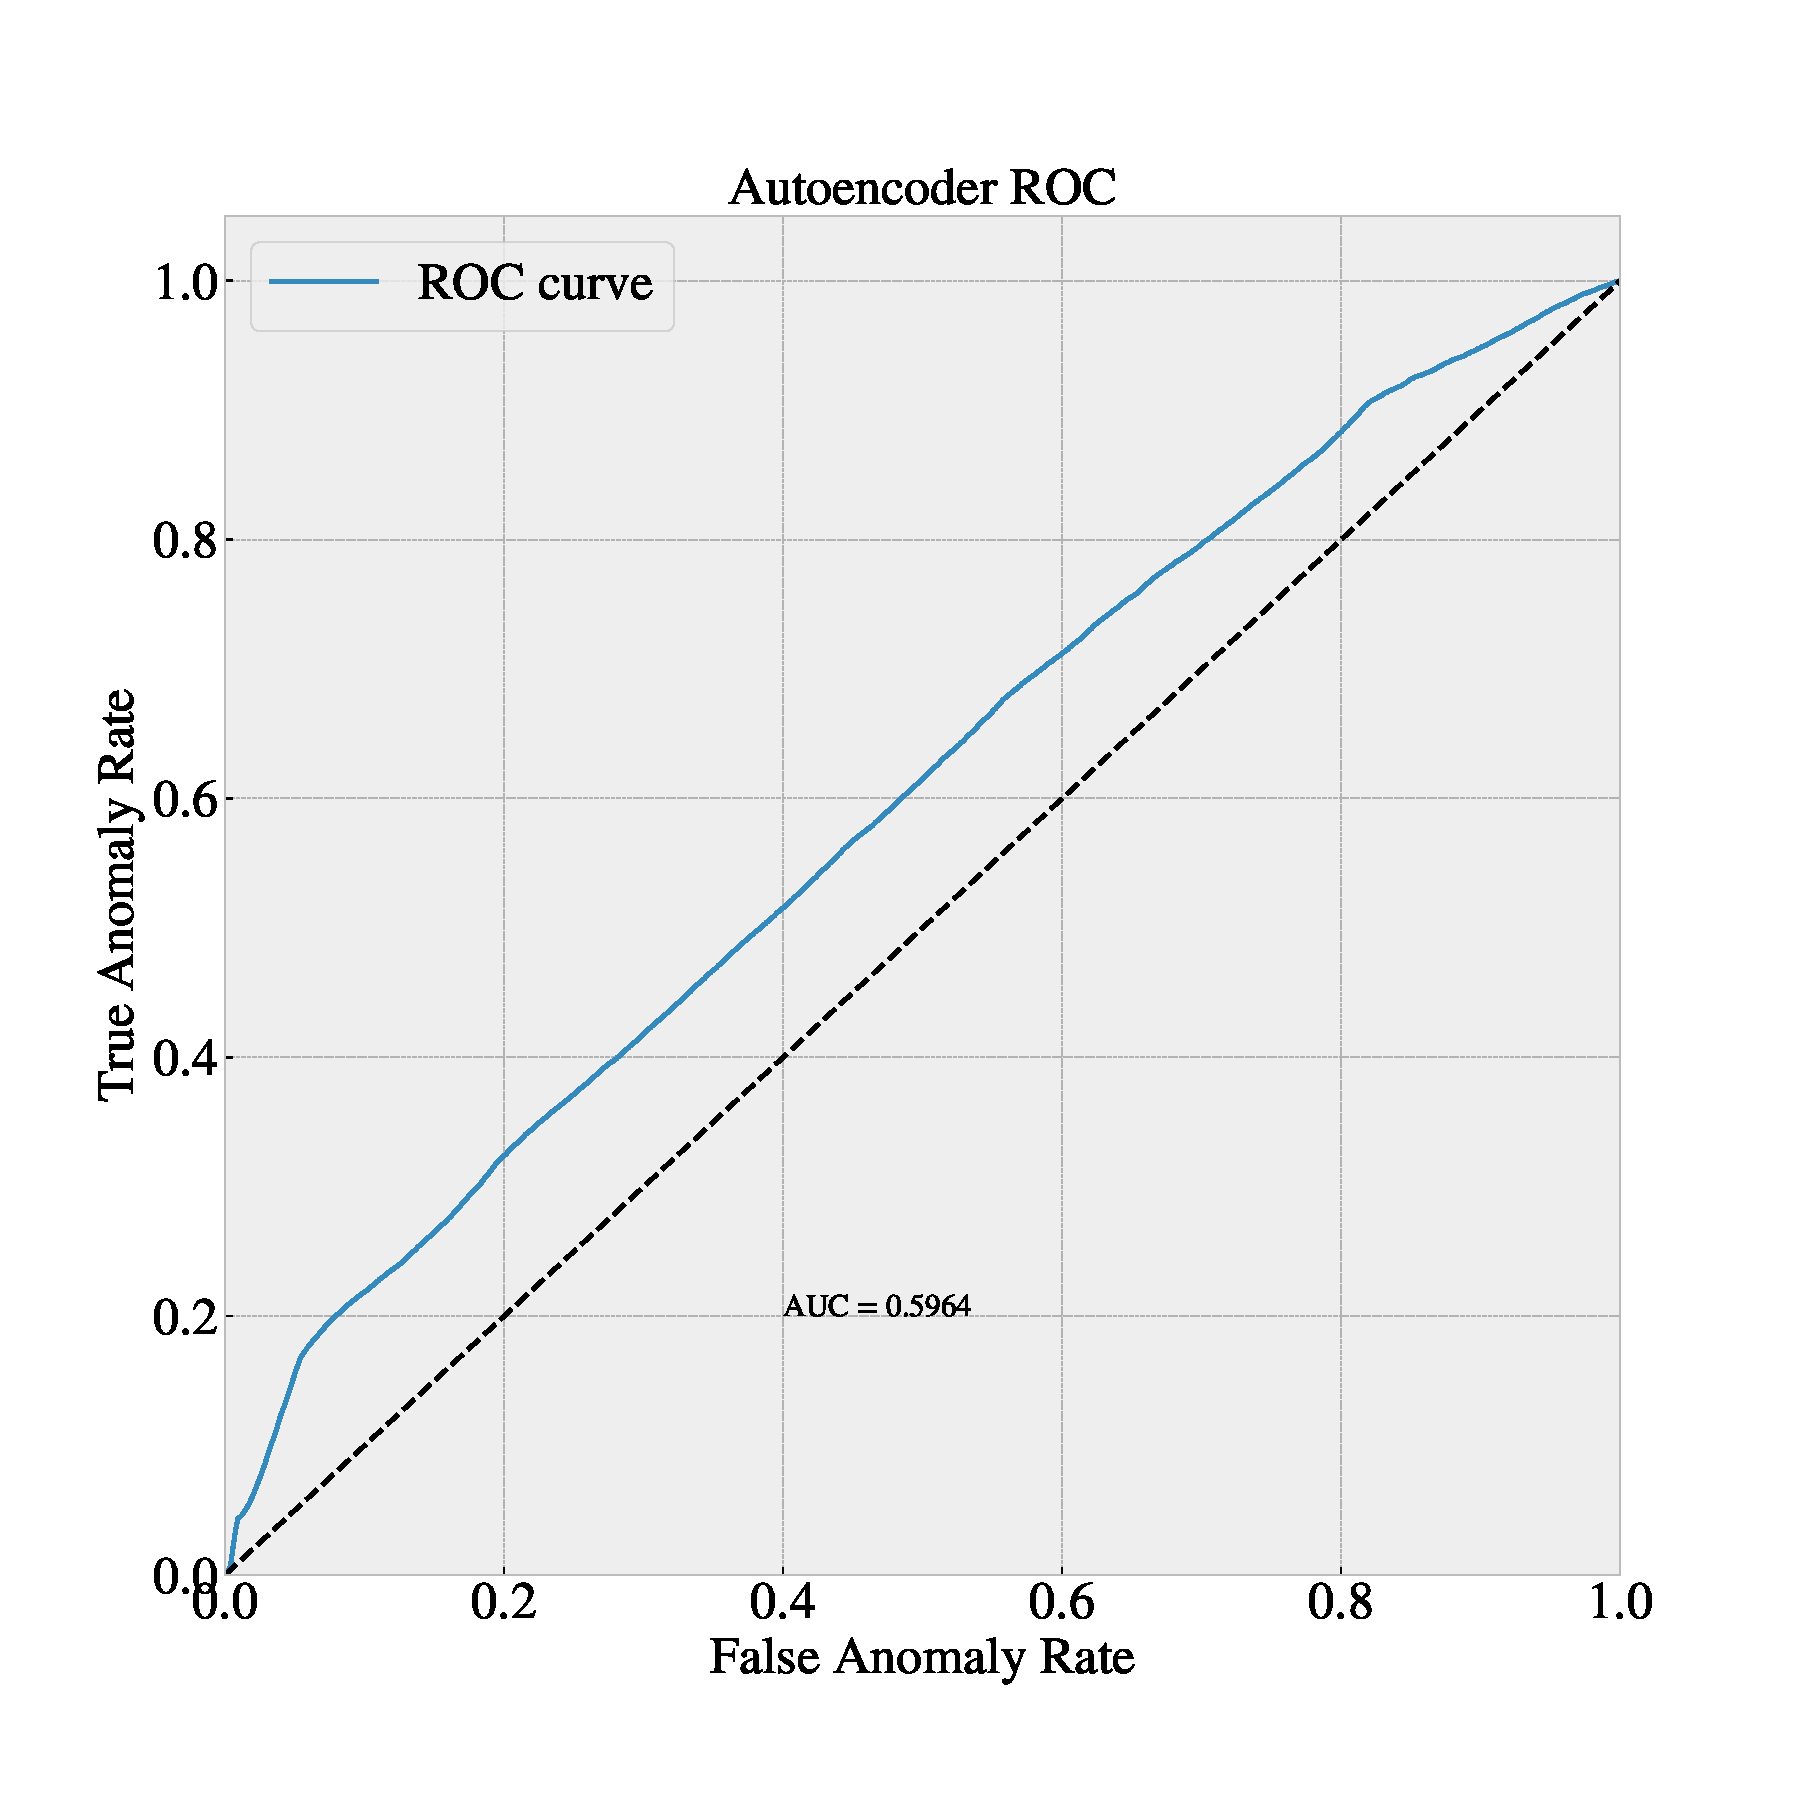
\includegraphics[width=0.46\textwidth]{figures/results/rocs/b_s_roc_curve_big_rmmanyfeats.pdf}
         \caption{ROC curve signal MC and background MC for big auto encoder using only 13 features.}
         \label{fig:s_b_big_roc_13}
\end{figure}



From figure \ref{fig:roc_sig_big_13feats} we observe that even with only 13 features, 
[njet60,  nbjet85, isOS,isSF,  mt2, met\_et,  , lep1\_pt,lep1\_E, lep1\_ptcone30, lep1\_etcone20, lep2\_pt,  lep2\_E, costhstar], the auto encoder struggles to separate background and signal MC. There are about 10 events around -0.3 MSE reconstruction error that it cannot match with background MC, but the rest of the data overlaps fairly well. The ROC score for the auto encoder was around 0.59, which only slightly better than for the dataset with all 33 features. \par

A third option is to change the scaling and look at its effect on the handling of data. The previous models have all used MinMax scaling to scale the data, where as this model used standard scaling instead. Using standard scaling I found the following results.

\begin{figure}[H]
     \centering
         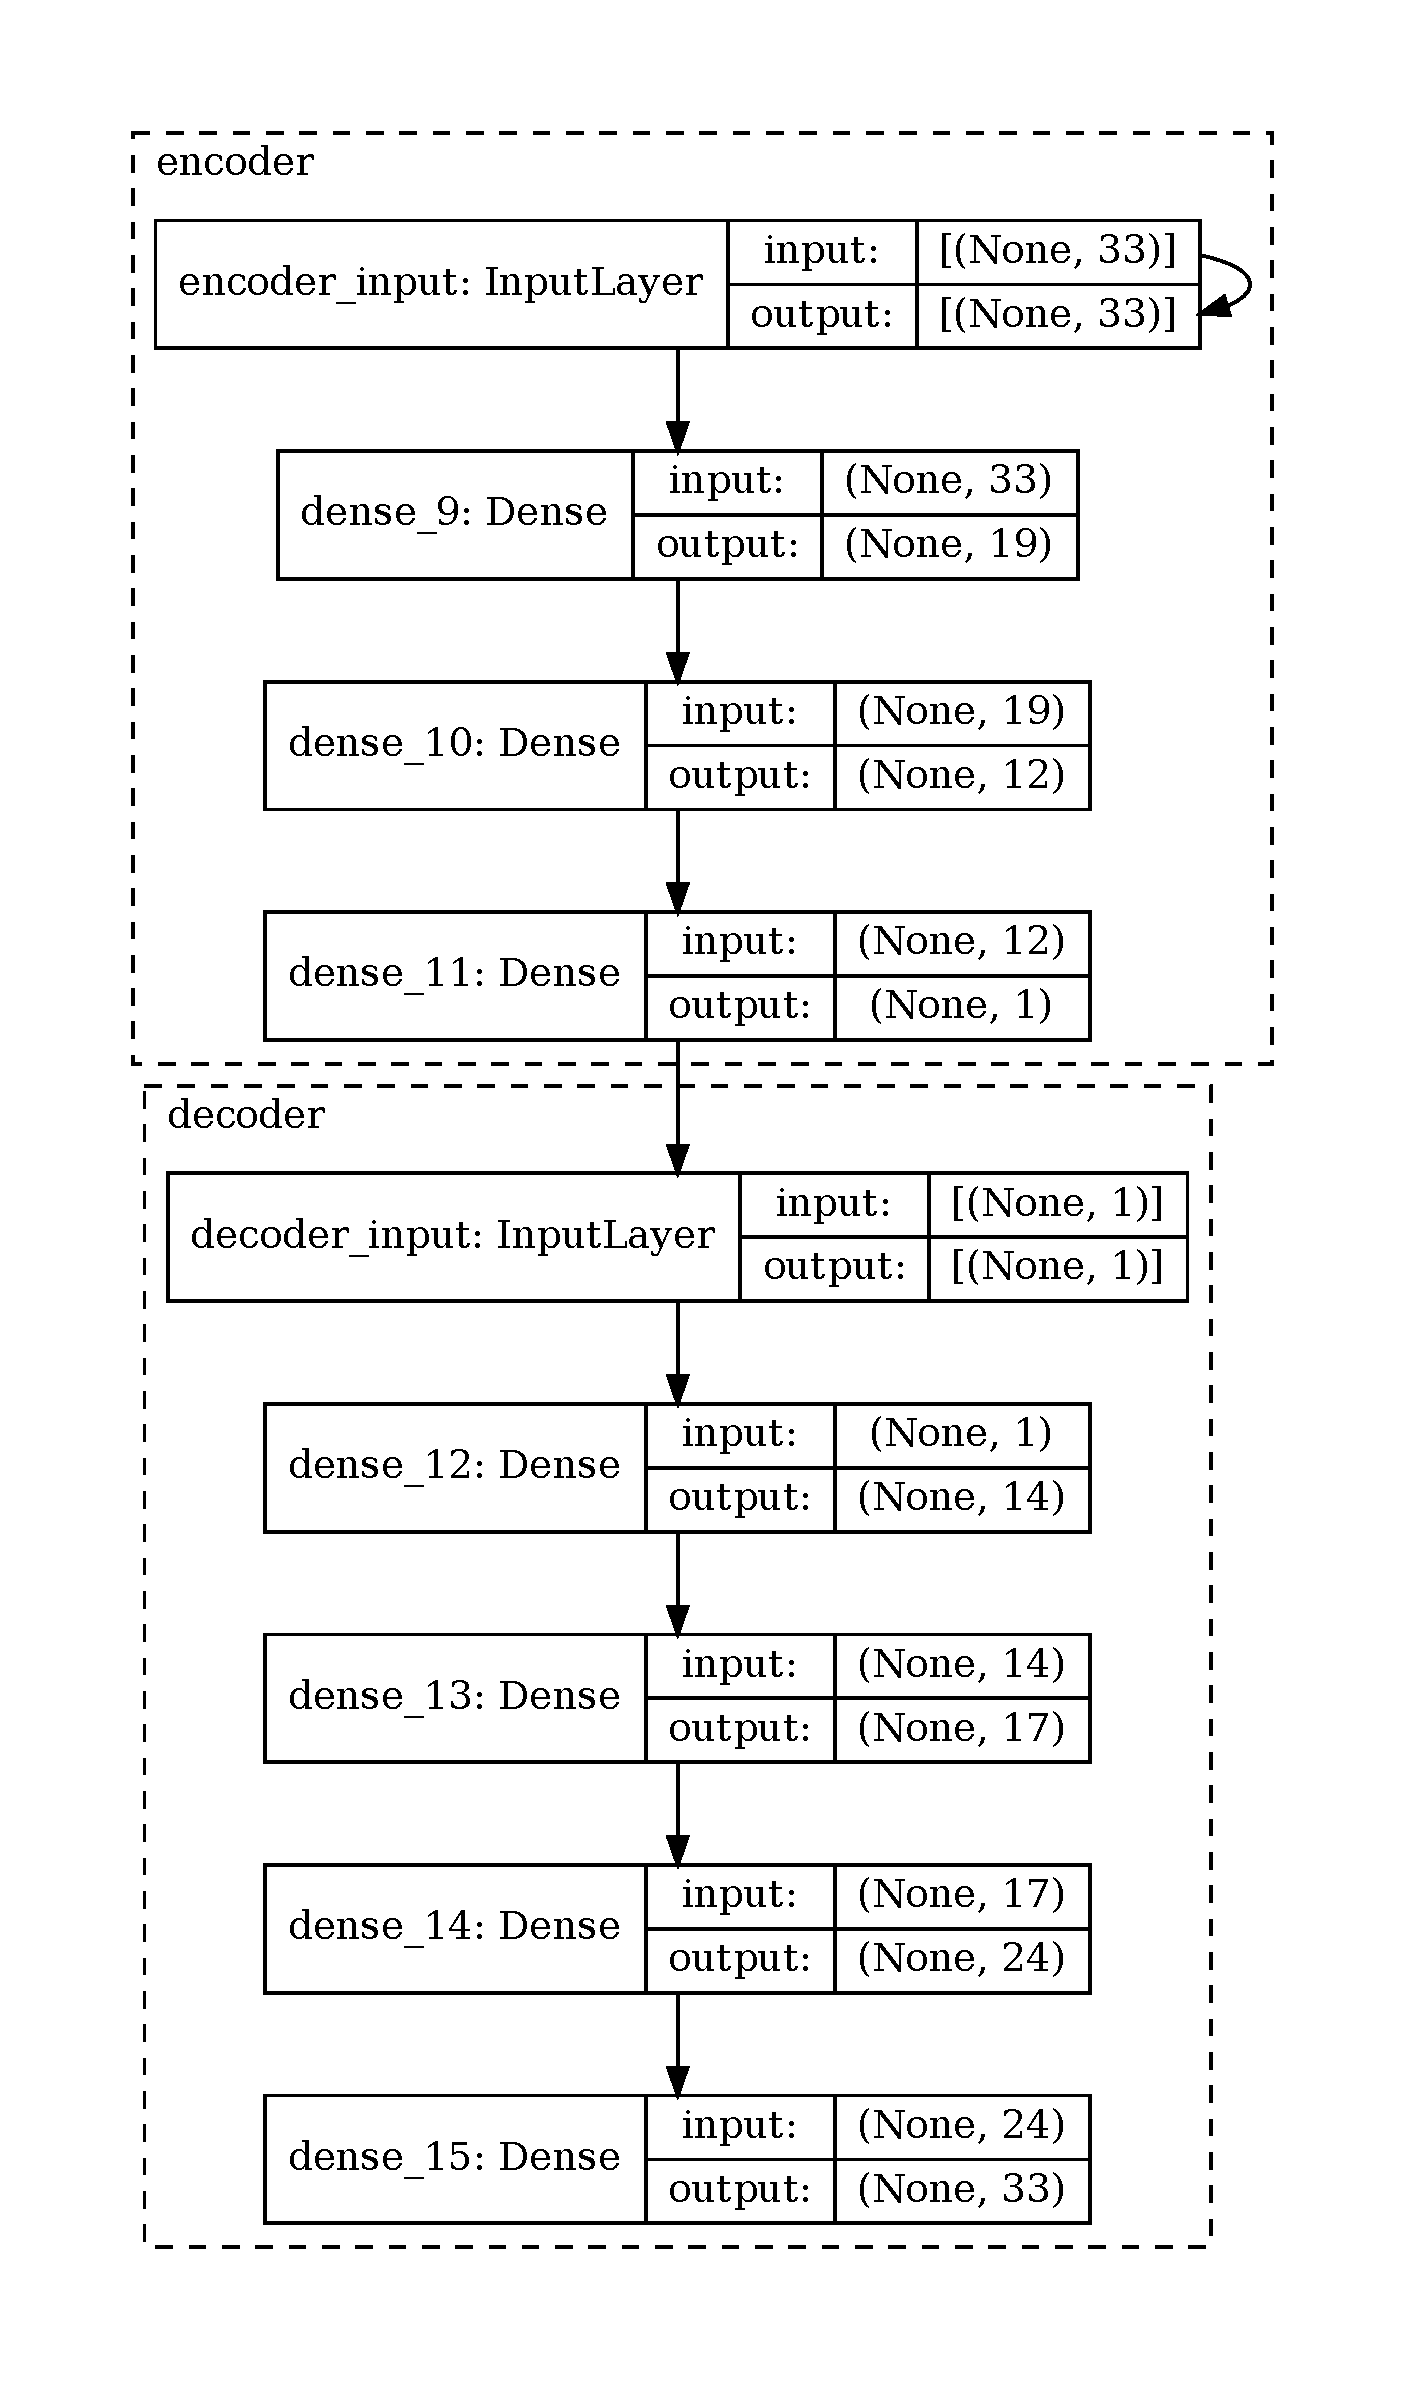
\includegraphics[width=0.46\textwidth]{figures/results/models/ae_model_plot_big_rm3feats_standard_propsigbacksplit.pdf}
         \caption{Auto encoder architecture after tuning of hyper parameters using standard scaling on the datasets. }
     \label{fig:ae_big_standard}
\end{figure}

In figure \ref{fig:ae_big_standard} we have the architecture for the auto encoder after hyper parameter tuning where the datasets are scaled using standard scaling. The hyperparameters were as follows. The activation functions for the encoder were tanh on all 4 layers. The activation functions for the decoder were leakyrelu for the first two layers and tanh for the last two layers. The kernel regularization, activation regularization and leaky relu alpha parameter were all 0.01, and the learning rate as 0.0015. The model was trained with 15 epochs.

\begin{figure}[H]
     \centering
         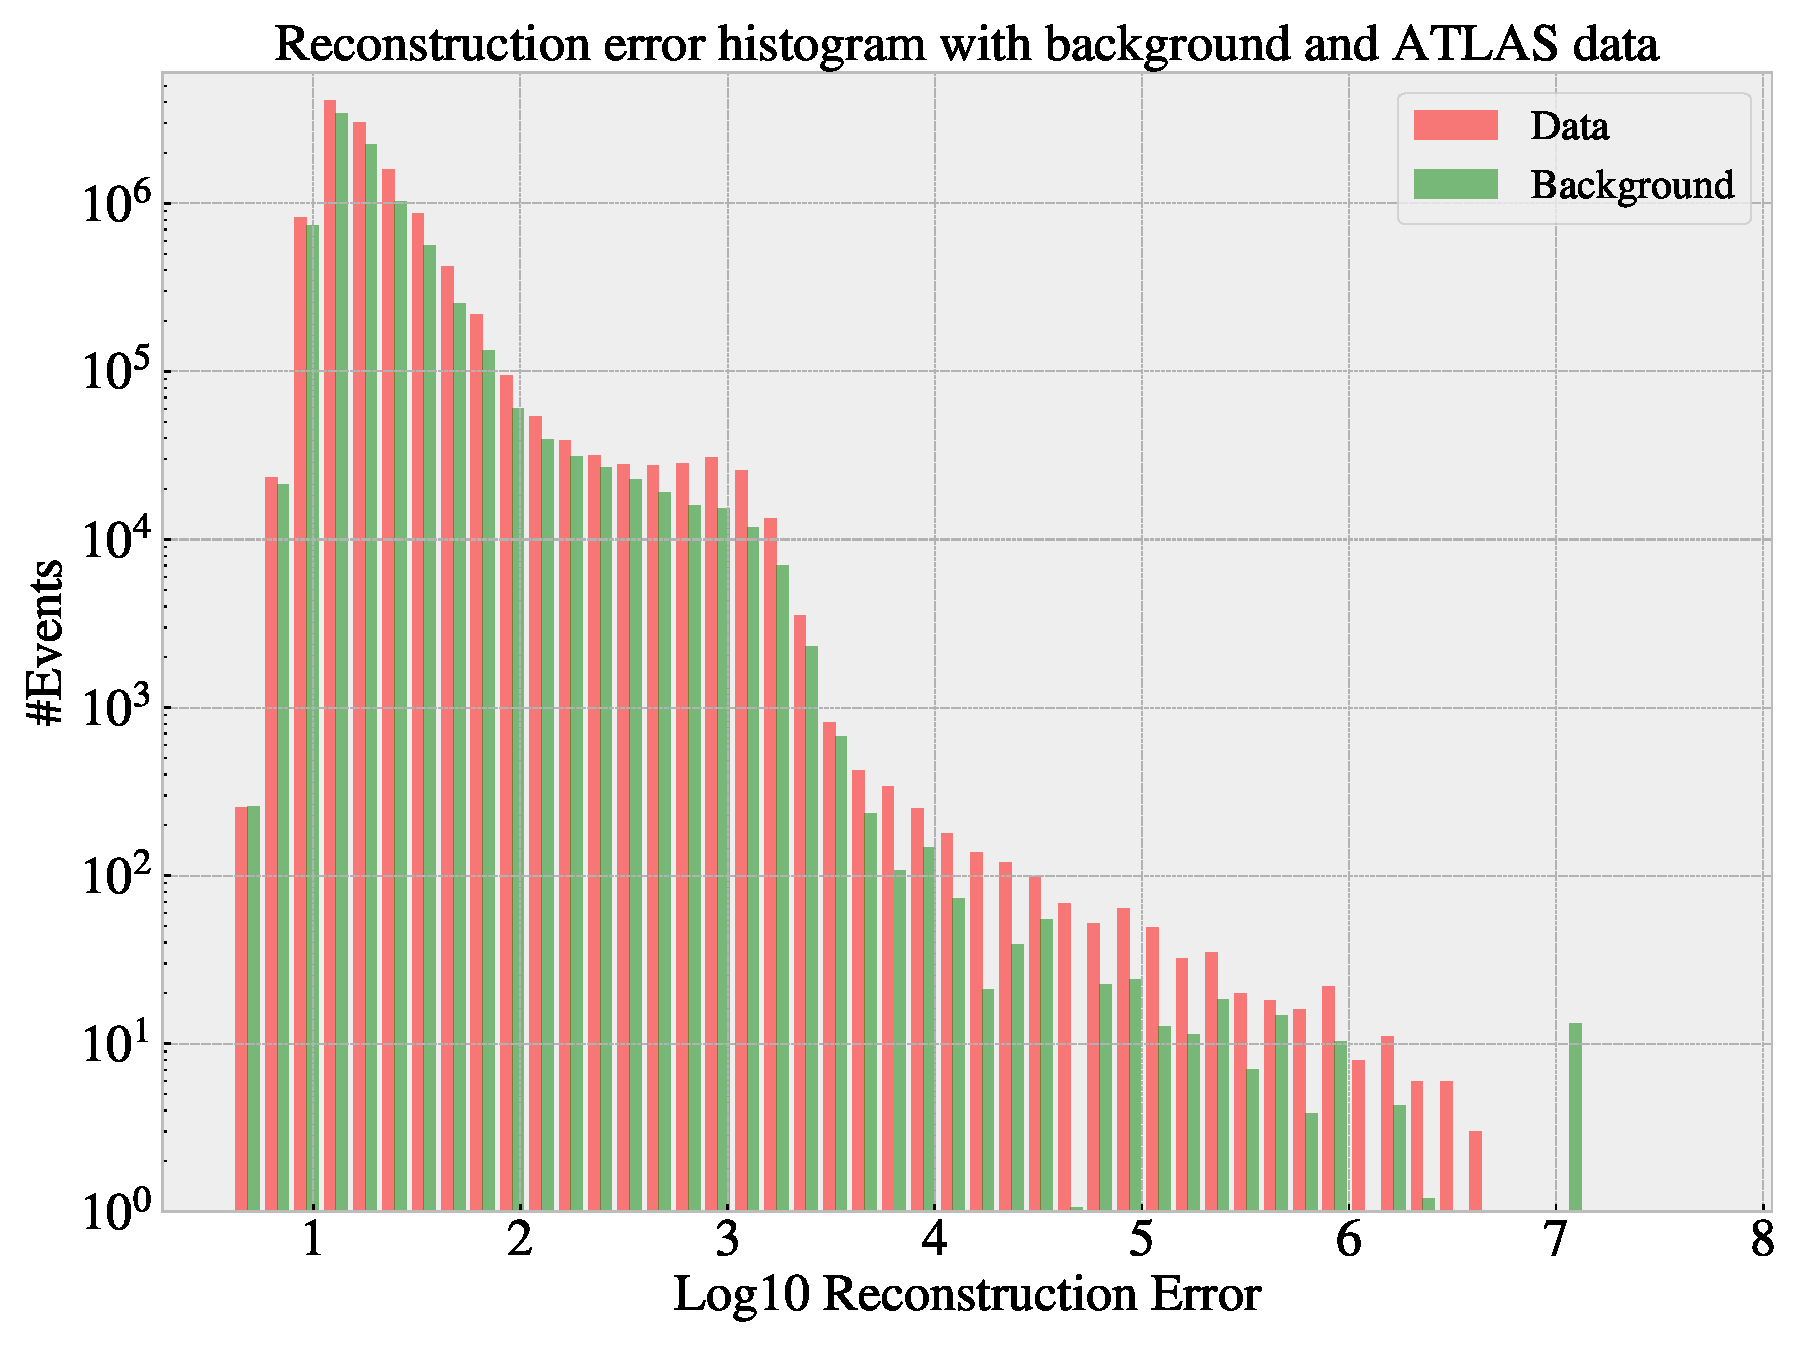
\includegraphics[width=0.46\textwidth]{figures/results/predictions/b_data_recon_big_rm3_feats_standard_propsigbacksplit.pdf}
         \caption{Histogram showing reconstruction error for ATLAS data and background MC for big auto encoder, using standard scaling.}
     \label{fig:data_b_big_pred_stand}
\end{figure}

In figure \ref{fig:data_b_big_pred_stand} we see that even though the reconstruction error for ATLAS data and background MC has a wide spread, it overlaps well, which indicates that the autoencoder learned to reproduce the standard model, even though some events where much harder to reproduce than others. 

\begin{figure}[H]
    \centering
    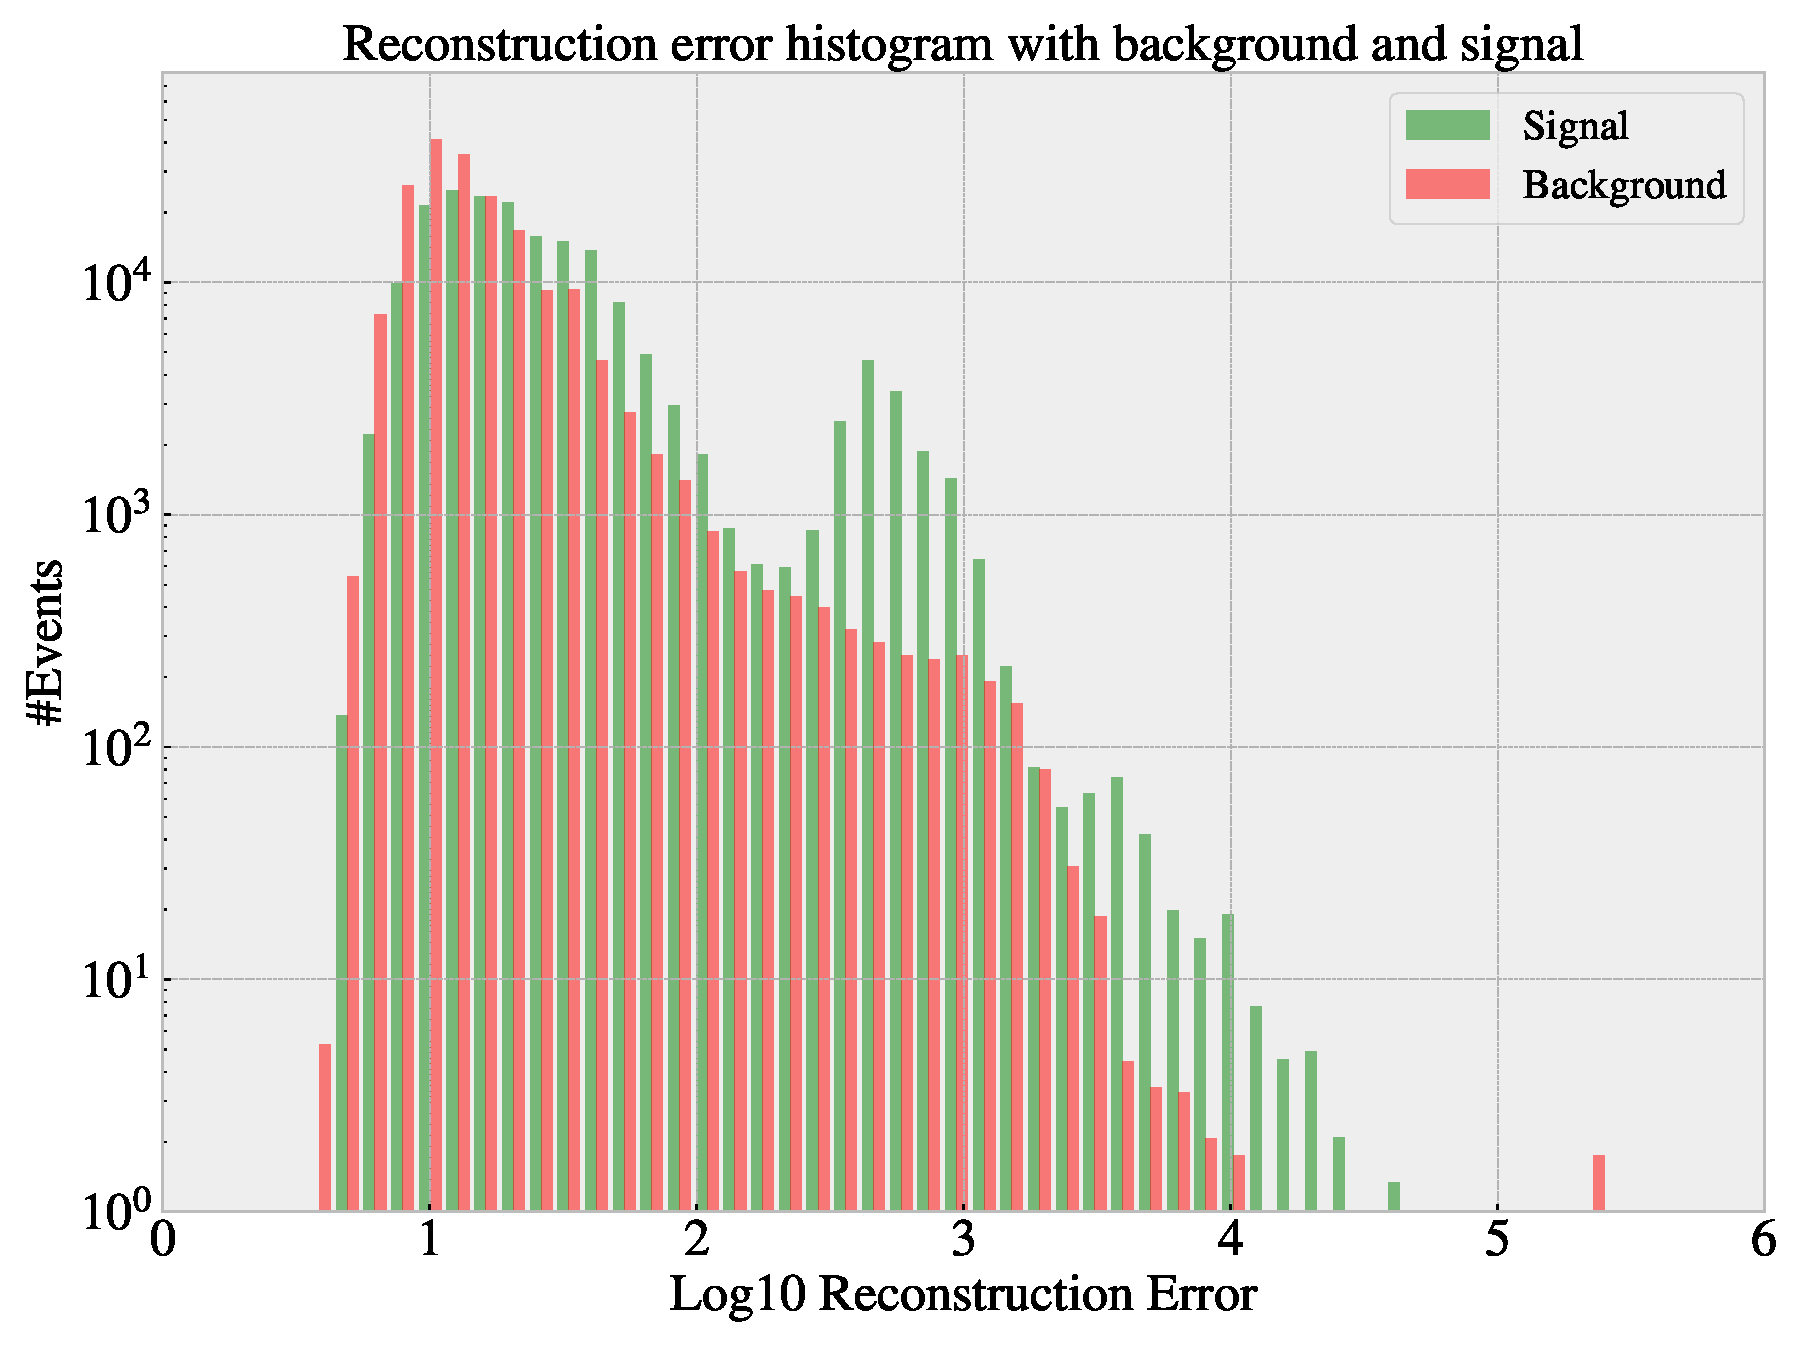
\includegraphics[width=0.46\textwidth]{figures/results/predictions/b_s_recon_big_rm3_feats_standard_propsigbacksplit_nolog_allsig_nogmumu.pdf}
    \caption{Reconstruction error of background MC and signal MC for big auto encoder, using standard scaling. }
    \label{fig:s_b_big_pred_stand}
\end{figure}

\begin{figure}[H]
    \centering
         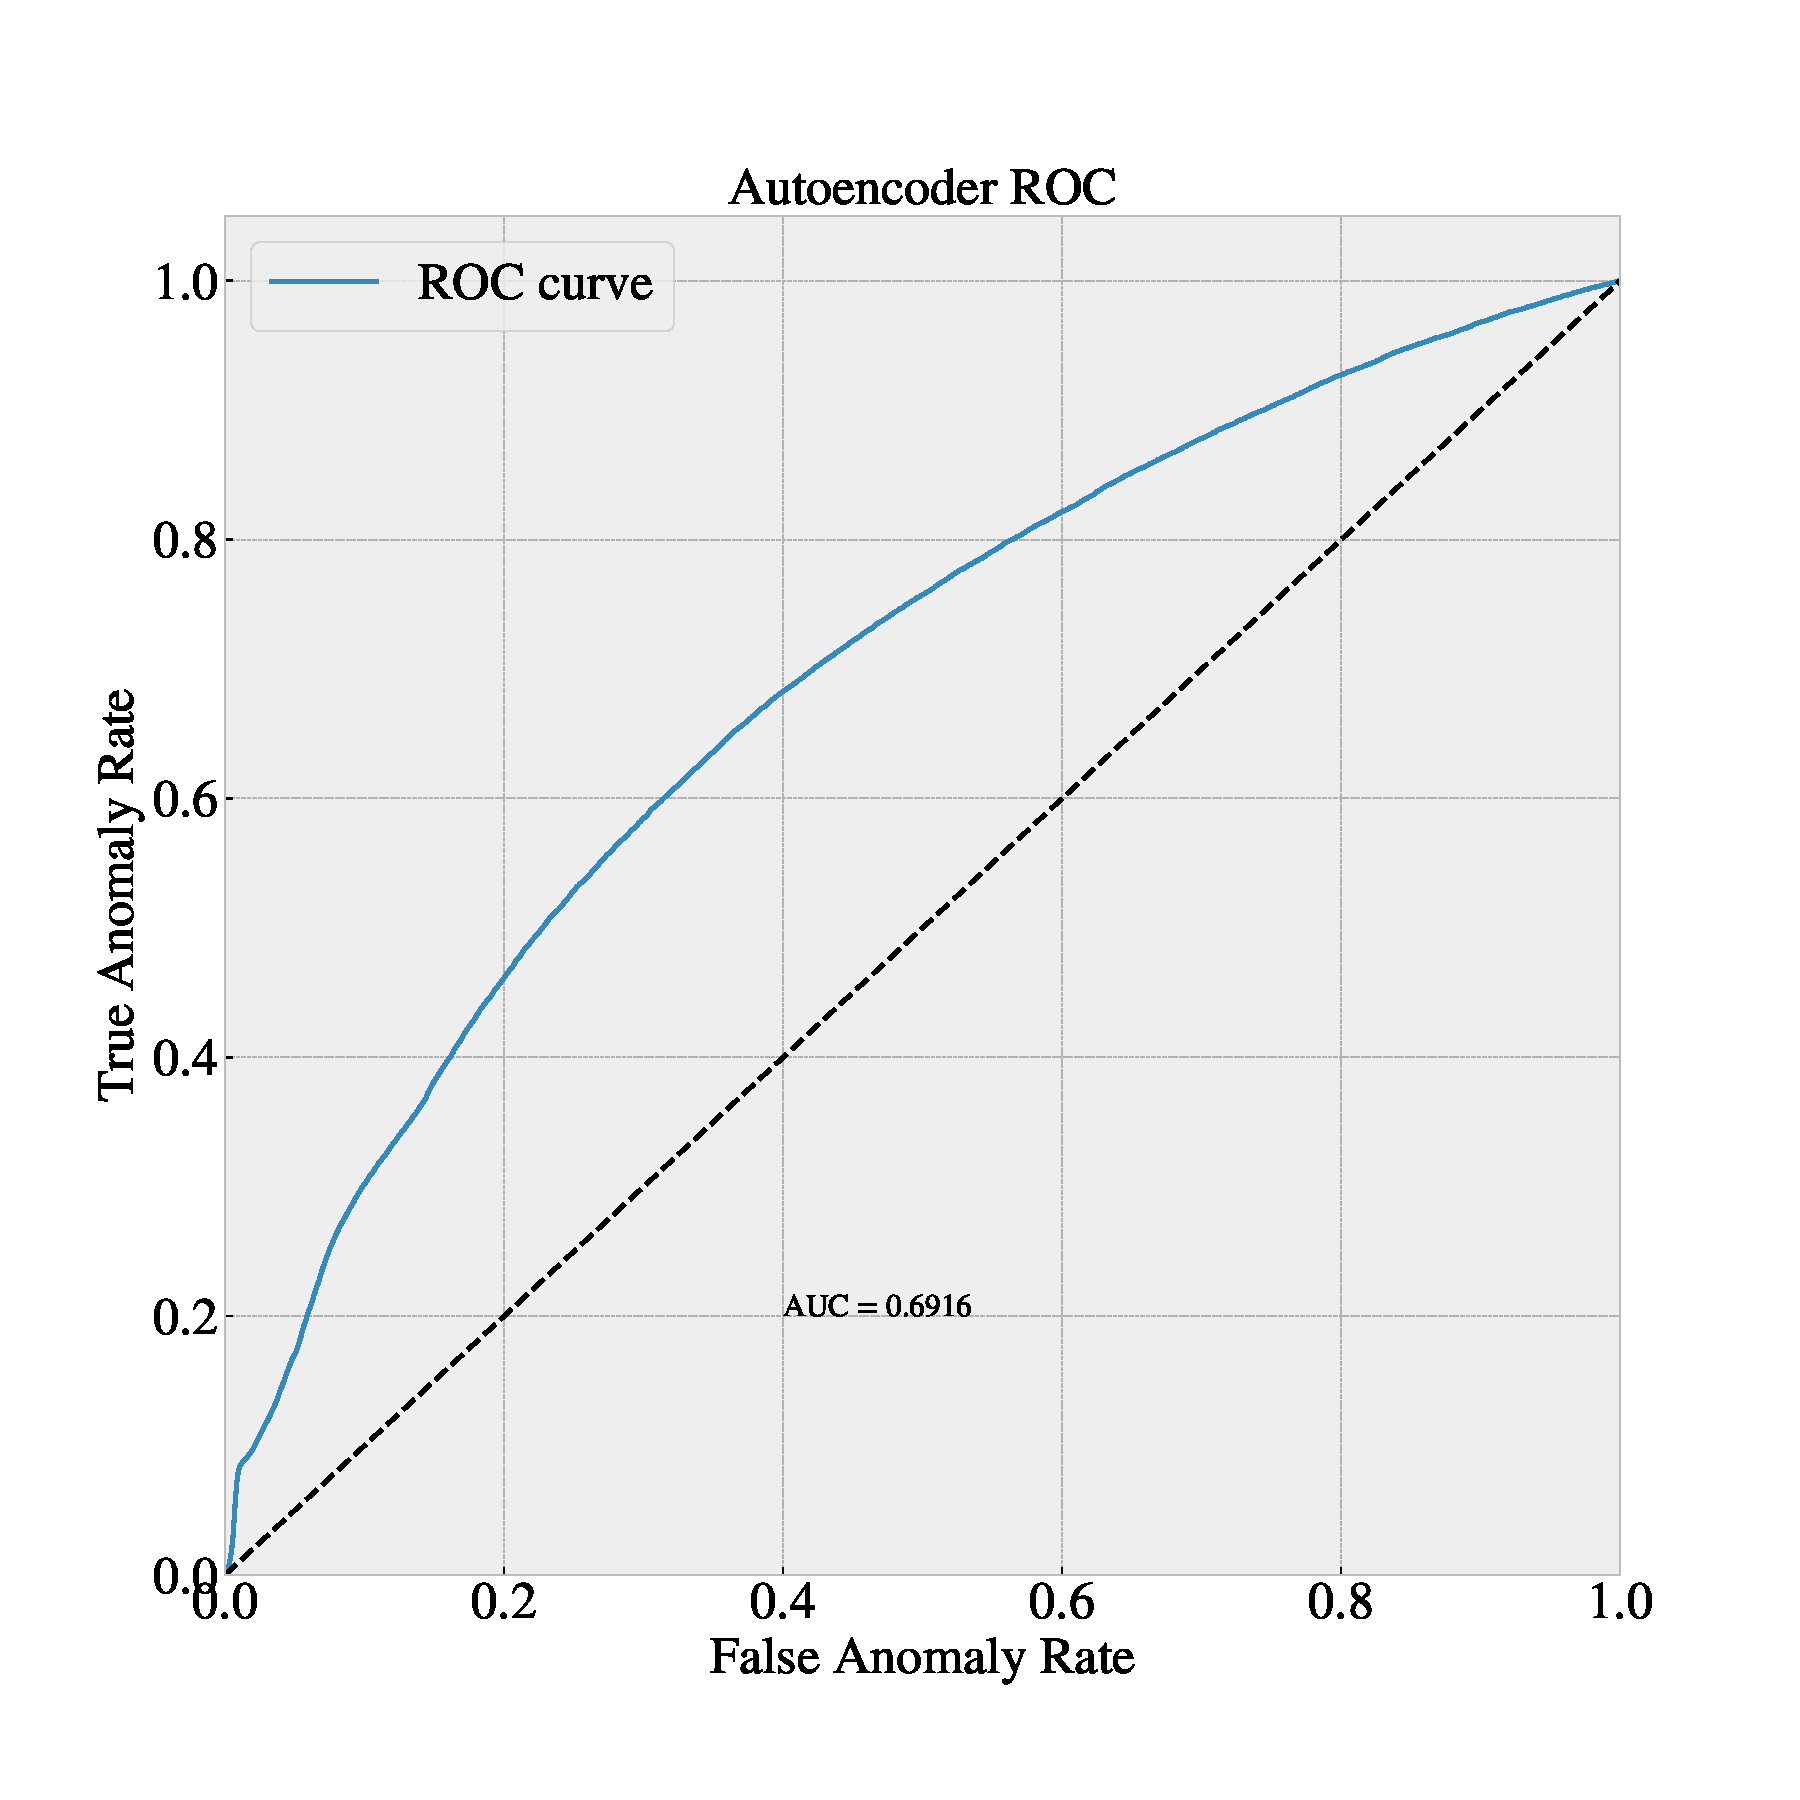
\includegraphics[width=0.46\textwidth]{figures/results/rocs/b_s_roc_curve_big_standard_allsig_nogmumu.pdf}
         \caption{ROC curve signal MC and background MC for big auto encoder, using standard scaling.}
         \label{fig:s_b_big_roc_stand}
\end{figure}



In figure \ref{fig:s_b_big_pred_stand} we observe that the model somewhat overlaps the background and signal MC, which the exception of a few thousand samples in the second peak. , so it appears here that the model manages to separate some signal events from the background MC. This model preformed better than the models using Min Max scaling, with a AUC score of about 0.69. \par 

\subsection{Discussion and possible ways forward}
There were several issues with training and tuning the model, much of which had to do with hardware. The background and signal MC data set alone was around 17 Gb of data. To do training, prediction and grid searches especially, GPU usage was needed. With Tensorflow's XLA\footnote{More on XLA \href{https://www.tensorflow.org/xla}{here}.} (Accelerated Linear Algebra), the algorithm got a speedup from 1 hour and 30 minutes to around 1 minute per epoch when training on 80\% of the background MC. Still, because of the enormous amount of data, the grid search had to be done using a smaller sample size. This was done by extracting 10 million events from the training set, randomly sampled, for training and 2 millions samples from the validation set (20\% of the hole background MC) for grid search validation. Thus each epoch only took 10-30 seconds, which allowed for many iterations of hyperparameter tuning. There is however the issue that the random sampling does accurately represent the SM background distribution, and thus the hyperparameters could very well have been even better tuned.  \par \par
It is also worth noting that the ROC curves and reconstruction error figure using the signal MC only in part shows how the auto encoder performs. The samples does not represent all possible new physics, and thus we can only conclude from our results that the auto encoder struggles to separate those signal MC samples. There might very well be possible signals that are much more different than the signal MC samples. This is however only true if the auto encoder actually learned some hidden relations between the features that are not easy to detect. \par \par
Another crucial point to make is that in the realm of machine learning, there are few guidelines for how the architecture should look. In this case with the auto encoder, the only requirement is that in the encoder the previous layers must have at least one more node than the one after, and in the decoder the layer after must have at least one more node than the one before it. With respect to the amount of layers, regularization of layers, bias or output, implementation of dropout layers or symmetry with regards to encoder and decoder architecture, an enormous hyper parameter search is the only way to find the ideal model. This bias that the designer of the given auto encoder brings is very hard to quantify, but is indeed crucial, and generates a gigantic pool of possibilities which, given enough time and resources could yield valuable insight. \par \par
Scaling also had an interesting impact on the output, as it appears that standard scaling allows for better detection of anomalies. Further research into the method made this even clearer. Background MC, signal MC and ATLAS data all have to be scaled with respect to the background MC, because if signal MC is used with background, the numerical values of background MC, signal MC and ATLAS data will be off, and biased towards the signal samples, which is a problem. \par \par


The choice of features also contributes to the effect of the auto encoder. The removal of the $d_0$ significance for both leptons was done by looking at the distribution of data and background MC by checking the difference between them, and was done by eye sight. This could certainly have been done better, for instance by checking  \par \par



From the results above it is clear that the auto encoder cannot be ruled out as a possibly good candidate for new physics search, as there are still many aspects that are not well understood. A good start would be to further study how the model learns to merge and reconstruct each feature, and if it quickly converges towards only focusing on one or a few main features. If this is better understood, then maybe the construction of certain features in the preparation of the background MC and ATLAS data could be made to handle this better. It could very well be that certain features or combinations of certain features are two similar for the algorithm to tell them apart. Another point of interest is the relation between number of features and complexity of the architecture. From the models tested above, it would appear that a stacked and more complex auto encoder is needed for the algorithm to learn to reproduce the dataset. It is also not clear if a symmetric architecture is more ideal than a non symmetric architecture, and a hyper parameter search with this included could yield interesting results. \par \par

%It is not well understood how the hyper parameters are affecting each other, and in relation to the auto encoder, it would be interesting to further analyze the balance between tuning the hyperparameters for good reconstruction and good separation. This also brings us to the definition of the problem it self. The method aims to use reconstruction as means of separating out anomalies. But there are some flaws here, some of which are already mentioned. Should one aims strictly for the best reconstruction error overlap, or should one add other metrics to slightly guide the network. 



\begin{itemize}
    \item Difference between broad and narrow search
    \item Bias 
    \item bias with features to choose
    \item difference of how well the model detects different signal models in mc data signals
    \item any interesting in actual data?
    \item difference in scaling
    \item tuning effect
    \item optimizing tensorflow code with use of autoclustering and possibly mixing floating point precision. 
    \item the use of roc curves, and the validity of what they say
    \item test if removing mll and mt2 makes a difference
    
\end{itemize}


\section{Conclusion}
This report attempted to create an auto encoder that manages to high accuracy reconstruct standard model processes based on training done on background MC and with poor reconstruction on collective anomalies given as signal MC samples. Several models where tuned using Keras-Tuner to get the optimal hyperparameters, and whilst all of the models successfully managed to have good overlap between background MC and ATLAS Open data, most of 


\clearpage
\newpage
\mbox{~}
\onecolumngrid
\printbibliography

\newpage
\appendix
\section{Features}\label{appendix:features}
% Define new columns types 
\newcolumntype{L}[1]{>{\raggedright\arraybackslash}p{#1}} % left fixed width
\newcolumntype{C}[1]{>{\centering\arraybackslash}p{#1}} % center fixed width
\newcolumntype{R}[1]{>{\raggedleft\arraybackslash}p{#1}} % flush right fixed width
\begin{table}[H]
    % \setlength{\tabcolsep}{15pt}
    \renewcommand{\arraystretch}{1.3}
    \begin{center}
    \caption{Features and their description \cite{ATL-OREACH-PUB-2020-001}}
    \begin{tabular}{|C{4.5cm}|C{4.5cm}|L{9.5cm}|} \hline
    
    Feature & Type & Description \\ \hline
    njet20 & int & Number of jets with $p_T > 20$ GeV\\ \hline
    njet60 & int & Number of jets with $p_T > 60$ GeV  \\ \hline
    nbjet60 & int & Number of b-jets with $p_T > 60$ GeV  \\ \hline
    nbjet70 & int & Number of b-jets with   \\ \hline
    nbjet77 & int & Number of b-jets with   \\ \hline
    nbjet85 & int & Number of b-jets with   \\ \hline
    isOS  & int & 1 if leptons have opposite charge, 0 if leptons have same charge \\ \hline
    isSF & int & 1 if leptons are of same flavor, 0 is leptons are of different flavor, flavor code 11 is electron, flavor code 13 is muon \\ \hline
    mll & float & Invariant mass of the two leptons \\ \hline
    mt2 & float & The maximal lower bound on the mass of each member of a
    pair of identical parent particles which, if pairproduced at a hadron collider, could have each
    undergone a two-body decay into (i) a visible
    particle (or collection of particles) and (ii) an
    invisible object of hypothesised mass $\chi$\cite{Lester_2011}.\\ \hline
    met\_et & float & Transverse energy of the missing momentum vector \\ \hline
    met\_phi & float & Azimuthal angle of the missing momentum vector\\ \hline
    lep\_flav & vector<int> & Flavor of the lepton, 11 for electron and 13 for muon \\ \hline
    lep\_pt & vector<float> & Vector containing transverse momentum for the leptons \\ \hline
    lep\_eta & vector<float> & Vector containing pseudo-rapidity , $\eta$, for the leptons \\ \hline
    lep\_phi & vector<float> & Vector containing azimuthal angle, $\phi$, for the leptons \\ \hline
    lep\_E & vector<float> & Vector containing the energy for the leptons \\ \hline
    lep\_ptcone30 & vector<float>  & Vector containing scalar sum of track $p_T$ in a cone of $R=0.3$ around lepton, used for tracking isolation \\ \hline
    lep\_etcone20 & vector<float>  & Vector containing scalar sum of track $E_T$ in a cone of $R=0.2$ around lepton, used for calorimeter isolation \\ \hline
    lep\_trackd0pvunbiased  & vector<float> & $d_0$ of track associated to lepton at point of closest approach (p.c.a.)\\ \hline
    lep\_tracksigd0pvunbiased & vector<float> & $d_0$ significance of the track associated to lepton at the p.c.a.\\ \hline
    lep\_isTightID & vector<bool> & Vector containing boolean indicating whether leptons satisfies tight ID reconstruction criteria\\ \hline
    lep\_z0 & vector<float> & Vector containing z-coordinate of the track associated for the leptons wrt. primary vertex \\ \hline
    
    channelNumber & int & Data sample ID\\\hline
    costhstar & float & Cosine of dilepton decay angle\\ \hline
    weight & float & MC sample weight \\ \hline
    category & string & SM or BSM category \\ \hline
    physdescr & string & MC process name \\ \hline
    isSignal & int & 1 if category is a BSM signal, 0 if the category is SM background \\ \hline
            
    \end{tabular}
    \label{tab:feature_table}
  \end{center}
\end{table}



\end{document}